\documentclass{book}
\usepackage[a4paper,top=2.5cm,bottom=2.5cm,left=2.5cm,right=2.5cm]{geometry}
\usepackage{makeidx}
\usepackage{natbib}
\usepackage{graphicx}
\usepackage{multicol}
\usepackage{float}
\usepackage{listings}
\usepackage{color}
\usepackage{ifthen}
\usepackage[table]{xcolor}
\usepackage{textcomp}
\usepackage{alltt}
\usepackage{ifpdf}
\ifpdf
\usepackage[pdftex,
            pagebackref=true,
            colorlinks=true,
            linkcolor=blue,
            unicode
           ]{hyperref}
\else
\usepackage[ps2pdf,
            pagebackref=true,
            colorlinks=true,
            linkcolor=blue,
            unicode
           ]{hyperref}
\usepackage{pspicture}
\fi
\usepackage[utf8]{inputenc}
\usepackage{mathptmx}
\usepackage[scaled=.90]{helvet}
\usepackage{courier}
\usepackage{sectsty}
\usepackage[titles]{tocloft}
\usepackage{doxygen}
\lstset{language=C++,inputencoding=utf8,basicstyle=\footnotesize,breaklines=true,breakatwhitespace=true,tabsize=8,numbers=left }
\makeindex
\setcounter{tocdepth}{3}
\renewcommand{\footrulewidth}{0.4pt}
\renewcommand{\familydefault}{\sfdefault}
\hfuzz=15pt
\setlength{\emergencystretch}{15pt}
\hbadness=750
\tolerance=750
\begin{document}
\hypersetup{pageanchor=false,citecolor=blue}
\begin{titlepage}
\vspace*{7cm}
\begin{center}
{\Large Calculatrice -\/ L\-O21 \\[1ex]\large 1.\-0 }\\
\vspace*{1cm}
{\large Generated by Doxygen 1.8.1}\\
\vspace*{0.5cm}
{\small Tue Jun 12 2012 22:36:17}\\
\end{center}
\end{titlepage}
\clearemptydoublepage
\pagenumbering{roman}
\tableofcontents
\clearemptydoublepage
\pagenumbering{arabic}
\hypersetup{pageanchor=true,citecolor=blue}
\chapter{L\-O21-\/calculatrice}
\label{md_README}
\hypertarget{md_README}{}
calculatrice notation polonaise inversée

Singleton Composite (expression) //\-N\-O\-N template methode (differnete facon d'évaluer un littéral command pathern (ctr Z) 
\chapter{Class Index}
\section{Class Hierarchy}
This inheritance list is sorted roughly, but not completely, alphabetically\-:\begin{DoxyCompactList}
\item \contentsline{section}{Calculatrice}{\pageref{class_calculatrice}}{}
\item \contentsline{section}{Commande}{\pageref{class_commande}}{}
\begin{DoxyCompactList}
\item \contentsline{section}{Commande\-Basic}{\pageref{class_commande_basic}}{}
\item \contentsline{section}{Commande\-Eval}{\pageref{class_commande_eval}}{}
\item \contentsline{section}{Commande\-Swap}{\pageref{class_commande_swap}}{}
\end{DoxyCompactList}
\item \contentsline{section}{Constante}{\pageref{class_constante}}{}
\begin{DoxyCompactList}
\item \contentsline{section}{C\-Complexe}{\pageref{class_c_complexe}}{}
\item \contentsline{section}{C\-Entier}{\pageref{class_c_entier}}{}
\item \contentsline{section}{C\-Expression}{\pageref{class_c_expression}}{}
\item \contentsline{section}{C\-Rationnel}{\pageref{class_c_rationnel}}{}
\item \contentsline{section}{C\-Reel}{\pageref{class_c_reel}}{}
\end{DoxyCompactList}
\item \contentsline{section}{Ecriture\-Dom}{\pageref{class_ecriture_dom}}{}
\item \contentsline{section}{Pile}{\pageref{class_pile}}{}
\item \contentsline{section}{Xml\-\_\-\-Dom}{\pageref{class_xml___dom}}{}
\end{DoxyCompactList}

\chapter{Class Index}
\section{Class List}
Here are the classes, structs, unions and interfaces with brief descriptions\-:\begin{DoxyCompactList}
\item\contentsline{section}{\hyperlink{class_calculatrice}{Calculatrice} \\*\hyperlink{class_calculatrice}{Calculatrice} class }{\pageref{class_calculatrice}}{}
\item\contentsline{section}{\hyperlink{class_c_complexe}{C\-Complexe} \\*\hyperlink{class_c_complexe}{C\-Complexe} class }{\pageref{class_c_complexe}}{}
\item\contentsline{section}{\hyperlink{class_c_entier}{C\-Entier} \\*\hyperlink{class_c_entier}{C\-Entier} class }{\pageref{class_c_entier}}{}
\item\contentsline{section}{\hyperlink{class_c_expression}{C\-Expression} \\*\hyperlink{class_c_expression}{C\-Expression} class }{\pageref{class_c_expression}}{}
\item\contentsline{section}{\hyperlink{class_commande}{Commande} \\*\hyperlink{class_commande}{Commande} class }{\pageref{class_commande}}{}
\item\contentsline{section}{\hyperlink{class_commande_basic}{Commande\-Basic} \\*\hyperlink{class_commande_basic}{Commande\-Basic} class }{\pageref{class_commande_basic}}{}
\item\contentsline{section}{\hyperlink{class_commande_eval}{Commande\-Eval} \\*\hyperlink{class_commande_eval}{Commande\-Eval} class }{\pageref{class_commande_eval}}{}
\item\contentsline{section}{\hyperlink{class_commande_swap}{Commande\-Swap} \\*\hyperlink{class_commande_swap}{Commande\-Swap} class }{\pageref{class_commande_swap}}{}
\item\contentsline{section}{\hyperlink{class_constante}{Constante} \\*\hyperlink{class_constante}{Constante} class }{\pageref{class_constante}}{}
\item\contentsline{section}{\hyperlink{class_c_rationnel}{C\-Rationnel} \\*\hyperlink{class_c_rationnel}{C\-Rationnel} class }{\pageref{class_c_rationnel}}{}
\item\contentsline{section}{\hyperlink{class_c_reel}{C\-Reel} \\*\hyperlink{class_c_reel}{C\-Reel} class }{\pageref{class_c_reel}}{}
\item\contentsline{section}{\hyperlink{class_ecriture_dom}{Ecriture\-Dom} \\*\hyperlink{class_ecriture_dom}{Ecriture\-Dom} class }{\pageref{class_ecriture_dom}}{}
\item\contentsline{section}{\hyperlink{class_pile}{Pile} \\*\hyperlink{class_pile}{Pile} class }{\pageref{class_pile}}{}
\item\contentsline{section}{\hyperlink{class_xml___dom}{Xml\-\_\-\-Dom} \\*\hyperlink{class_xml___dom}{Xml\-\_\-\-Dom} class }{\pageref{class_xml___dom}}{}
\end{DoxyCompactList}

\chapter{Class Documentation}
\hypertarget{class_calculatrice}{\section{Calculatrice Class Reference}
\label{class_calculatrice}\index{Calculatrice@{Calculatrice}}
}


\hyperlink{class_calculatrice}{Calculatrice} class.  




{\ttfamily \#include $<$calculatrice.\-h$>$}

\subsection*{Public Slots}
\begin{DoxyCompactItemize}
\item 
void \hyperlink{class_calculatrice_a1a45487e6b9c8c81960f53e8a1f08401}{creer\-Tab} ()
\begin{DoxyCompactList}\small\item\em cree un nouvel onglet \end{DoxyCompactList}\item 
void \hyperlink{class_calculatrice_a47a89aec6c63b04b64cf1cb9c742739f}{detruire\-Tab} (int index)
\begin{DoxyCompactList}\small\item\em detruit l'onglet actif \end{DoxyCompactList}\item 
void \hyperlink{class_calculatrice_a62b04788444746c01b1c99d8b1daeb50}{ecrire} (const Q\-String \&a)
\begin{DoxyCompactList}\small\item\em ecrire dans le champ texte \end{DoxyCompactList}\item 
void \hyperlink{class_calculatrice_a07bc4dfff9dbc5e2805873c470b64609}{effacer} ()
\begin{DoxyCompactList}\small\item\em effacer le dernier caract�re du champ texte \end{DoxyCompactList}\item 
void \hyperlink{class_calculatrice_a0698e23c0033882dfd4f1c92c819fb76}{envoyer} ()
\begin{DoxyCompactList}\small\item\em Envoyer le contenu du champ texte pour etre analyser. \end{DoxyCompactList}\item 
void \hyperlink{class_calculatrice_a4b1d40e63040fb49b730d25b97f11147}{afficher} (int max)
\begin{DoxyCompactList}\small\item\em afficher la pile active \end{DoxyCompactList}\item 
void \hyperlink{class_calculatrice_ae04068faaa66847c3f318c018824a277}{annuler} ()
\begin{DoxyCompactList}\small\item\em annule la derni�re commande \end{DoxyCompactList}\item 
void \hyperlink{class_calculatrice_ac9fea1beaab60d0c73c017a5d225a56c}{retablir} ()
\begin{DoxyCompactList}\small\item\em retabli la derni�re commande \end{DoxyCompactList}\item 
void \hyperlink{class_calculatrice_af9e1bd08361e13a0d68da5ff6ebb79d5}{redimentionner} (bool)
\begin{DoxyCompactList}\small\item\em redimentionne la fenetre de la \hyperlink{class_calculatrice}{Calculatrice} \end{DoxyCompactList}\end{DoxyCompactItemize}
\subsection*{Public Member Functions}
\begin{DoxyCompactItemize}
\item 
\hyperlink{class_pile}{Pile} $\ast$ \hyperlink{class_calculatrice_a48f797c689bd992a8fee2404bbd75896}{pile\-Active} ()
\begin{DoxyCompactList}\small\item\em Recherche et retourne la pile active. \end{DoxyCompactList}\item 
void \hyperlink{class_calculatrice_a5641a5ff484e68bb4917143a52086179}{chg\-Entier} ()
\begin{DoxyCompactList}\small\item\em Active l'option Entier. \end{DoxyCompactList}\item 
void \hyperlink{class_calculatrice_ab932c8e399ffc9ab8c3edf17b69a93b0}{chg\-Rationnel} ()
\begin{DoxyCompactList}\small\item\em Active l'option Rationnel. \end{DoxyCompactList}\item 
void \hyperlink{class_calculatrice_ae7331880310b197bee6d4576a1aeaf34}{chg\-Reel} ()
\begin{DoxyCompactList}\small\item\em Active l'option Reel. \end{DoxyCompactList}\item 
void \hyperlink{class_calculatrice_a8eaad4eaf0ef211152d8207dea5893bd}{chg\-Complexe} ()
\begin{DoxyCompactList}\small\item\em Active l'option Complexe. \end{DoxyCompactList}\item 
void \hyperlink{class_calculatrice_ab399629989ffbfb8a5a58110fa399372}{chg\-Degre} ()
\begin{DoxyCompactList}\small\item\em Active l'option Degre. \end{DoxyCompactList}\item 
void \hyperlink{class_calculatrice_a26d589ddd37ddfa604dbaec6b5cbcb36}{chg\-Radian} ()
\begin{DoxyCompactList}\small\item\em Active l'option Radian. \end{DoxyCompactList}\item 
void \hyperlink{class_calculatrice_a164d12758f93d6b7d038a12155d445b2}{sauvegarde} ()
\begin{DoxyCompactList}\small\item\em Enregistre l'etat actuelle des piles et options de la calculatrice. \end{DoxyCompactList}\end{DoxyCompactItemize}
\subsection*{Static Public Member Functions}
\begin{DoxyCompactItemize}
\item 
static \hyperlink{class_calculatrice}{Calculatrice} $\ast$ \hyperlink{class_calculatrice_a727f903b74a7761efca79d2360c74a34}{get\-Instance} ()
\begin{DoxyCompactList}\small\item\em Initialisation d'un objet \hyperlink{class_calculatrice}{Calculatrice} si aucun n'existe. \end{DoxyCompactList}\item 
static void \hyperlink{class_calculatrice_afadb6109e631a4050e299720723b467a}{kill} ()
\begin{DoxyCompactList}\small\item\em Detruit l'unique objet \hyperlink{class_calculatrice}{Calculatrice}. \end{DoxyCompactList}\end{DoxyCompactItemize}
\subsection*{Public Attributes}
\begin{DoxyCompactItemize}
\item 
std\-::vector$<$ \hyperlink{class_pile}{Pile} $\ast$ $>$ \hyperlink{class_calculatrice_ae45c1dccda6c9ba95aa43e65fb566e1e}{onglet}
\begin{DoxyCompactList}\small\item\em Tableau des pointeurs de piles. \end{DoxyCompactList}\end{DoxyCompactItemize}


\subsection{Detailed Description}
\hyperlink{class_calculatrice}{Calculatrice} class. 

fenetre principale de la calculatrice. 

\subsection{Member Function Documentation}
\hypertarget{class_calculatrice_a4b1d40e63040fb49b730d25b97f11147}{\index{Calculatrice@{Calculatrice}!afficher@{afficher}}
\index{afficher@{afficher}!Calculatrice@{Calculatrice}}
\subsubsection[{afficher}]{\setlength{\rightskip}{0pt plus 5cm}void Calculatrice\-::afficher (
\begin{DoxyParamCaption}
\item[{int}]{max}
\end{DoxyParamCaption}
)\hspace{0.3cm}{\ttfamily [slot]}}}\label{class_calculatrice_a4b1d40e63040fb49b730d25b97f11147}


afficher la pile active 


\begin{DoxyParams}{Parameters}
{\em max} & nombre d'element � afficher. \\
\hline
\end{DoxyParams}
\begin{DoxySeeAlso}{See also}
\hyperlink{class_calculatrice_a62b04788444746c01b1c99d8b1daeb50}{ecrire()}, \hyperlink{class_calculatrice_a07bc4dfff9dbc5e2805873c470b64609}{effacer()} et \hyperlink{class_calculatrice_a0698e23c0033882dfd4f1c92c819fb76}{envoyer()} 
\end{DoxySeeAlso}
\hypertarget{class_calculatrice_ae04068faaa66847c3f318c018824a277}{\index{Calculatrice@{Calculatrice}!annuler@{annuler}}
\index{annuler@{annuler}!Calculatrice@{Calculatrice}}
\subsubsection[{annuler}]{\setlength{\rightskip}{0pt plus 5cm}void Calculatrice\-::annuler (
\begin{DoxyParamCaption}
{}
\end{DoxyParamCaption}
)\hspace{0.3cm}{\ttfamily [slot]}}}\label{class_calculatrice_ae04068faaa66847c3f318c018824a277}


annule la derni�re commande 

\begin{DoxySeeAlso}{See also}
\hyperlink{class_calculatrice_ac9fea1beaab60d0c73c017a5d225a56c}{retablir()} 
\end{DoxySeeAlso}
\hypertarget{class_calculatrice_a8eaad4eaf0ef211152d8207dea5893bd}{\index{Calculatrice@{Calculatrice}!chg\-Complexe@{chg\-Complexe}}
\index{chg\-Complexe@{chg\-Complexe}!Calculatrice@{Calculatrice}}
\subsubsection[{chg\-Complexe}]{\setlength{\rightskip}{0pt plus 5cm}void Calculatrice\-::chg\-Complexe (
\begin{DoxyParamCaption}
{}
\end{DoxyParamCaption}
)}}\label{class_calculatrice_a8eaad4eaf0ef211152d8207dea5893bd}


Active l'option Complexe. 

\begin{DoxySeeAlso}{See also}
\hyperlink{class_calculatrice_a5641a5ff484e68bb4917143a52086179}{chg\-Entier()}, \hyperlink{class_calculatrice_ab932c8e399ffc9ab8c3edf17b69a93b0}{chg\-Rationnel()}, \hyperlink{class_calculatrice_ae7331880310b197bee6d4576a1aeaf34}{chg\-Reel()}, \hyperlink{class_calculatrice_ab399629989ffbfb8a5a58110fa399372}{chg\-Degre()}, \hyperlink{class_calculatrice_a26d589ddd37ddfa604dbaec6b5cbcb36}{chg\-Radian()} et \hyperlink{class_calculatrice_a164d12758f93d6b7d038a12155d445b2}{sauvegarde()} 
\end{DoxySeeAlso}
\hypertarget{class_calculatrice_ab399629989ffbfb8a5a58110fa399372}{\index{Calculatrice@{Calculatrice}!chg\-Degre@{chg\-Degre}}
\index{chg\-Degre@{chg\-Degre}!Calculatrice@{Calculatrice}}
\subsubsection[{chg\-Degre}]{\setlength{\rightskip}{0pt plus 5cm}void Calculatrice\-::chg\-Degre (
\begin{DoxyParamCaption}
{}
\end{DoxyParamCaption}
)}}\label{class_calculatrice_ab399629989ffbfb8a5a58110fa399372}


Active l'option Degre. 

\begin{DoxySeeAlso}{See also}
\hyperlink{class_calculatrice_a5641a5ff484e68bb4917143a52086179}{chg\-Entier()}, \hyperlink{class_calculatrice_ab932c8e399ffc9ab8c3edf17b69a93b0}{chg\-Rationnel()}, \hyperlink{class_calculatrice_ae7331880310b197bee6d4576a1aeaf34}{chg\-Reel()}, \hyperlink{class_calculatrice_a8eaad4eaf0ef211152d8207dea5893bd}{chg\-Complexe()}, \hyperlink{class_calculatrice_a26d589ddd37ddfa604dbaec6b5cbcb36}{chg\-Radian()} et \hyperlink{class_calculatrice_a164d12758f93d6b7d038a12155d445b2}{sauvegarde()} 
\end{DoxySeeAlso}
\hypertarget{class_calculatrice_a5641a5ff484e68bb4917143a52086179}{\index{Calculatrice@{Calculatrice}!chg\-Entier@{chg\-Entier}}
\index{chg\-Entier@{chg\-Entier}!Calculatrice@{Calculatrice}}
\subsubsection[{chg\-Entier}]{\setlength{\rightskip}{0pt plus 5cm}void Calculatrice\-::chg\-Entier (
\begin{DoxyParamCaption}
{}
\end{DoxyParamCaption}
)}}\label{class_calculatrice_a5641a5ff484e68bb4917143a52086179}


Active l'option Entier. 

\begin{DoxySeeAlso}{See also}
\hyperlink{class_calculatrice_ab932c8e399ffc9ab8c3edf17b69a93b0}{chg\-Rationnel()}, \hyperlink{class_calculatrice_ae7331880310b197bee6d4576a1aeaf34}{chg\-Reel()}, \hyperlink{class_calculatrice_a8eaad4eaf0ef211152d8207dea5893bd}{chg\-Complexe()}, \hyperlink{class_calculatrice_ab399629989ffbfb8a5a58110fa399372}{chg\-Degre()}, \hyperlink{class_calculatrice_a26d589ddd37ddfa604dbaec6b5cbcb36}{chg\-Radian()} et \hyperlink{class_calculatrice_a164d12758f93d6b7d038a12155d445b2}{sauvegarde()} 
\end{DoxySeeAlso}
\hypertarget{class_calculatrice_a26d589ddd37ddfa604dbaec6b5cbcb36}{\index{Calculatrice@{Calculatrice}!chg\-Radian@{chg\-Radian}}
\index{chg\-Radian@{chg\-Radian}!Calculatrice@{Calculatrice}}
\subsubsection[{chg\-Radian}]{\setlength{\rightskip}{0pt plus 5cm}void Calculatrice\-::chg\-Radian (
\begin{DoxyParamCaption}
{}
\end{DoxyParamCaption}
)}}\label{class_calculatrice_a26d589ddd37ddfa604dbaec6b5cbcb36}


Active l'option Radian. 

\begin{DoxySeeAlso}{See also}
\hyperlink{class_calculatrice_a5641a5ff484e68bb4917143a52086179}{chg\-Entier()}, \hyperlink{class_calculatrice_ab932c8e399ffc9ab8c3edf17b69a93b0}{chg\-Rationnel()}, \hyperlink{class_calculatrice_ae7331880310b197bee6d4576a1aeaf34}{chg\-Reel()}, \hyperlink{class_calculatrice_a8eaad4eaf0ef211152d8207dea5893bd}{chg\-Complexe()}, \hyperlink{class_calculatrice_ab399629989ffbfb8a5a58110fa399372}{chg\-Degre()} et \hyperlink{class_calculatrice_a164d12758f93d6b7d038a12155d445b2}{sauvegarde()} 
\end{DoxySeeAlso}
\hypertarget{class_calculatrice_ab932c8e399ffc9ab8c3edf17b69a93b0}{\index{Calculatrice@{Calculatrice}!chg\-Rationnel@{chg\-Rationnel}}
\index{chg\-Rationnel@{chg\-Rationnel}!Calculatrice@{Calculatrice}}
\subsubsection[{chg\-Rationnel}]{\setlength{\rightskip}{0pt plus 5cm}void Calculatrice\-::chg\-Rationnel (
\begin{DoxyParamCaption}
{}
\end{DoxyParamCaption}
)}}\label{class_calculatrice_ab932c8e399ffc9ab8c3edf17b69a93b0}


Active l'option Rationnel. 

\begin{DoxySeeAlso}{See also}
\hyperlink{class_calculatrice_a5641a5ff484e68bb4917143a52086179}{chg\-Entier()}, \hyperlink{class_calculatrice_ae7331880310b197bee6d4576a1aeaf34}{chg\-Reel()}, \hyperlink{class_calculatrice_a8eaad4eaf0ef211152d8207dea5893bd}{chg\-Complexe()}, \hyperlink{class_calculatrice_ab399629989ffbfb8a5a58110fa399372}{chg\-Degre()}, \hyperlink{class_calculatrice_a26d589ddd37ddfa604dbaec6b5cbcb36}{chg\-Radian()} et \hyperlink{class_calculatrice_a164d12758f93d6b7d038a12155d445b2}{sauvegarde()} 
\end{DoxySeeAlso}
\hypertarget{class_calculatrice_ae7331880310b197bee6d4576a1aeaf34}{\index{Calculatrice@{Calculatrice}!chg\-Reel@{chg\-Reel}}
\index{chg\-Reel@{chg\-Reel}!Calculatrice@{Calculatrice}}
\subsubsection[{chg\-Reel}]{\setlength{\rightskip}{0pt plus 5cm}void Calculatrice\-::chg\-Reel (
\begin{DoxyParamCaption}
{}
\end{DoxyParamCaption}
)}}\label{class_calculatrice_ae7331880310b197bee6d4576a1aeaf34}


Active l'option Reel. 

\begin{DoxySeeAlso}{See also}
\hyperlink{class_calculatrice_a5641a5ff484e68bb4917143a52086179}{chg\-Entier()}, \hyperlink{class_calculatrice_ab932c8e399ffc9ab8c3edf17b69a93b0}{chg\-Rationnel()}, \hyperlink{class_calculatrice_a8eaad4eaf0ef211152d8207dea5893bd}{chg\-Complexe()}, \hyperlink{class_calculatrice_ab399629989ffbfb8a5a58110fa399372}{chg\-Degre()}, \hyperlink{class_calculatrice_a26d589ddd37ddfa604dbaec6b5cbcb36}{chg\-Radian()} et \hyperlink{class_calculatrice_a164d12758f93d6b7d038a12155d445b2}{sauvegarde()} 
\end{DoxySeeAlso}
\hypertarget{class_calculatrice_a1a45487e6b9c8c81960f53e8a1f08401}{\index{Calculatrice@{Calculatrice}!creer\-Tab@{creer\-Tab}}
\index{creer\-Tab@{creer\-Tab}!Calculatrice@{Calculatrice}}
\subsubsection[{creer\-Tab}]{\setlength{\rightskip}{0pt plus 5cm}void Calculatrice\-::creer\-Tab (
\begin{DoxyParamCaption}
{}
\end{DoxyParamCaption}
)\hspace{0.3cm}{\ttfamily [slot]}}}\label{class_calculatrice_a1a45487e6b9c8c81960f53e8a1f08401}


cree un nouvel onglet 

\begin{DoxySeeAlso}{See also}
\hyperlink{class_calculatrice_a47a89aec6c63b04b64cf1cb9c742739f}{detruire\-Tab()} 
\end{DoxySeeAlso}
\hypertarget{class_calculatrice_a47a89aec6c63b04b64cf1cb9c742739f}{\index{Calculatrice@{Calculatrice}!detruire\-Tab@{detruire\-Tab}}
\index{detruire\-Tab@{detruire\-Tab}!Calculatrice@{Calculatrice}}
\subsubsection[{detruire\-Tab}]{\setlength{\rightskip}{0pt plus 5cm}void Calculatrice\-::detruire\-Tab (
\begin{DoxyParamCaption}
\item[{int}]{index}
\end{DoxyParamCaption}
)\hspace{0.3cm}{\ttfamily [slot]}}}\label{class_calculatrice_a47a89aec6c63b04b64cf1cb9c742739f}


detruit l'onglet actif 


\begin{DoxyParams}{Parameters}
{\em index} & un integer (position de l'onglet) \\
\hline
\end{DoxyParams}
\begin{DoxySeeAlso}{See also}
\hyperlink{class_calculatrice_a1a45487e6b9c8c81960f53e8a1f08401}{creer\-Tab()} 
\end{DoxySeeAlso}
\hypertarget{class_calculatrice_a62b04788444746c01b1c99d8b1daeb50}{\index{Calculatrice@{Calculatrice}!ecrire@{ecrire}}
\index{ecrire@{ecrire}!Calculatrice@{Calculatrice}}
\subsubsection[{ecrire}]{\setlength{\rightskip}{0pt plus 5cm}void Calculatrice\-::ecrire (
\begin{DoxyParamCaption}
\item[{const Q\-String \&}]{a}
\end{DoxyParamCaption}
)\hspace{0.3cm}{\ttfamily [slot]}}}\label{class_calculatrice_a62b04788444746c01b1c99d8b1daeb50}


ecrire dans le champ texte 


\begin{DoxyParams}{Parameters}
{\em a} & une Q\-String. \\
\hline
\end{DoxyParams}
\begin{DoxySeeAlso}{See also}
\hyperlink{class_calculatrice_a07bc4dfff9dbc5e2805873c470b64609}{effacer()}, \hyperlink{class_calculatrice_a0698e23c0033882dfd4f1c92c819fb76}{envoyer()} et \hyperlink{class_calculatrice_a4b1d40e63040fb49b730d25b97f11147}{afficher()} 
\end{DoxySeeAlso}
\hypertarget{class_calculatrice_a07bc4dfff9dbc5e2805873c470b64609}{\index{Calculatrice@{Calculatrice}!effacer@{effacer}}
\index{effacer@{effacer}!Calculatrice@{Calculatrice}}
\subsubsection[{effacer}]{\setlength{\rightskip}{0pt plus 5cm}void Calculatrice\-::effacer (
\begin{DoxyParamCaption}
{}
\end{DoxyParamCaption}
)\hspace{0.3cm}{\ttfamily [slot]}}}\label{class_calculatrice_a07bc4dfff9dbc5e2805873c470b64609}


effacer le dernier caract�re du champ texte 

\begin{DoxySeeAlso}{See also}
\hyperlink{class_calculatrice_a62b04788444746c01b1c99d8b1daeb50}{ecrire()}, \hyperlink{class_calculatrice_a0698e23c0033882dfd4f1c92c819fb76}{envoyer()} et \hyperlink{class_calculatrice_a4b1d40e63040fb49b730d25b97f11147}{afficher()} 
\end{DoxySeeAlso}
\hypertarget{class_calculatrice_a0698e23c0033882dfd4f1c92c819fb76}{\index{Calculatrice@{Calculatrice}!envoyer@{envoyer}}
\index{envoyer@{envoyer}!Calculatrice@{Calculatrice}}
\subsubsection[{envoyer}]{\setlength{\rightskip}{0pt plus 5cm}void Calculatrice\-::envoyer (
\begin{DoxyParamCaption}
{}
\end{DoxyParamCaption}
)\hspace{0.3cm}{\ttfamily [slot]}}}\label{class_calculatrice_a0698e23c0033882dfd4f1c92c819fb76}


Envoyer le contenu du champ texte pour etre analyser. 

\begin{DoxySeeAlso}{See also}
\hyperlink{class_calculatrice_a62b04788444746c01b1c99d8b1daeb50}{ecrire()}, \hyperlink{class_calculatrice_a07bc4dfff9dbc5e2805873c470b64609}{effacer()} et \hyperlink{class_calculatrice_a4b1d40e63040fb49b730d25b97f11147}{afficher()} 
\end{DoxySeeAlso}
\hypertarget{class_calculatrice_a727f903b74a7761efca79d2360c74a34}{\index{Calculatrice@{Calculatrice}!get\-Instance@{get\-Instance}}
\index{get\-Instance@{get\-Instance}!Calculatrice@{Calculatrice}}
\subsubsection[{get\-Instance}]{\setlength{\rightskip}{0pt plus 5cm}static {\bf Calculatrice}$\ast$ Calculatrice\-::get\-Instance (
\begin{DoxyParamCaption}
{}
\end{DoxyParamCaption}
)\hspace{0.3cm}{\ttfamily [inline]}, {\ttfamily [static]}}}\label{class_calculatrice_a727f903b74a7761efca79d2360c74a34}


Initialisation d'un objet \hyperlink{class_calculatrice}{Calculatrice} si aucun n'existe. 

\begin{DoxyReturn}{Returns}
pointeur vers un objet \hyperlink{class_calculatrice}{Calculatrice} 
\end{DoxyReturn}
\begin{DoxySeeAlso}{See also}
\hyperlink{class_calculatrice_afadb6109e631a4050e299720723b467a}{kill()}, Calculatrice() et $\sim$\-Calculatrice() 
\end{DoxySeeAlso}
\hypertarget{class_calculatrice_afadb6109e631a4050e299720723b467a}{\index{Calculatrice@{Calculatrice}!kill@{kill}}
\index{kill@{kill}!Calculatrice@{Calculatrice}}
\subsubsection[{kill}]{\setlength{\rightskip}{0pt plus 5cm}static void Calculatrice\-::kill (
\begin{DoxyParamCaption}
{}
\end{DoxyParamCaption}
)\hspace{0.3cm}{\ttfamily [inline]}, {\ttfamily [static]}}}\label{class_calculatrice_afadb6109e631a4050e299720723b467a}


Detruit l'unique objet \hyperlink{class_calculatrice}{Calculatrice}. 

\begin{DoxySeeAlso}{See also}
\hyperlink{class_calculatrice_a727f903b74a7761efca79d2360c74a34}{get\-Instance()}, Calculatrice() et $\sim$\-Calculatrice() 
\end{DoxySeeAlso}
\hypertarget{class_calculatrice_a48f797c689bd992a8fee2404bbd75896}{\index{Calculatrice@{Calculatrice}!pile\-Active@{pile\-Active}}
\index{pile\-Active@{pile\-Active}!Calculatrice@{Calculatrice}}
\subsubsection[{pile\-Active}]{\setlength{\rightskip}{0pt plus 5cm}{\bf Pile} $\ast$ Calculatrice\-::pile\-Active (
\begin{DoxyParamCaption}
{}
\end{DoxyParamCaption}
)}}\label{class_calculatrice_a48f797c689bd992a8fee2404bbd75896}


Recherche et retourne la pile active. 

\begin{DoxyReturn}{Returns}
pointeur de pile active 
\end{DoxyReturn}
\hypertarget{class_calculatrice_af9e1bd08361e13a0d68da5ff6ebb79d5}{\index{Calculatrice@{Calculatrice}!redimentionner@{redimentionner}}
\index{redimentionner@{redimentionner}!Calculatrice@{Calculatrice}}
\subsubsection[{redimentionner}]{\setlength{\rightskip}{0pt plus 5cm}void Calculatrice\-::redimentionner (
\begin{DoxyParamCaption}
\item[{bool}]{t}
\end{DoxyParamCaption}
)\hspace{0.3cm}{\ttfamily [slot]}}}\label{class_calculatrice_af9e1bd08361e13a0d68da5ff6ebb79d5}


redimentionne la fenetre de la \hyperlink{class_calculatrice}{Calculatrice} 


\begin{DoxyParams}{Parameters}
{\em t} & boolean pour les deux positions. \\
\hline
\end{DoxyParams}
\hypertarget{class_calculatrice_ac9fea1beaab60d0c73c017a5d225a56c}{\index{Calculatrice@{Calculatrice}!retablir@{retablir}}
\index{retablir@{retablir}!Calculatrice@{Calculatrice}}
\subsubsection[{retablir}]{\setlength{\rightskip}{0pt plus 5cm}void Calculatrice\-::retablir (
\begin{DoxyParamCaption}
{}
\end{DoxyParamCaption}
)\hspace{0.3cm}{\ttfamily [slot]}}}\label{class_calculatrice_ac9fea1beaab60d0c73c017a5d225a56c}


retabli la derni�re commande 

\begin{DoxySeeAlso}{See also}
\hyperlink{class_calculatrice_ae04068faaa66847c3f318c018824a277}{annuler()} 
\end{DoxySeeAlso}
\hypertarget{class_calculatrice_a164d12758f93d6b7d038a12155d445b2}{\index{Calculatrice@{Calculatrice}!sauvegarde@{sauvegarde}}
\index{sauvegarde@{sauvegarde}!Calculatrice@{Calculatrice}}
\subsubsection[{sauvegarde}]{\setlength{\rightskip}{0pt plus 5cm}void Calculatrice\-::sauvegarde (
\begin{DoxyParamCaption}
{}
\end{DoxyParamCaption}
)}}\label{class_calculatrice_a164d12758f93d6b7d038a12155d445b2}


Enregistre l'etat actuelle des piles et options de la calculatrice. 

\begin{DoxySeeAlso}{See also}
\hyperlink{class_calculatrice_a5641a5ff484e68bb4917143a52086179}{chg\-Entier()}, \hyperlink{class_calculatrice_ab932c8e399ffc9ab8c3edf17b69a93b0}{chg\-Rationnel()}, \hyperlink{class_calculatrice_ae7331880310b197bee6d4576a1aeaf34}{chg\-Reel()}, \hyperlink{class_calculatrice_a8eaad4eaf0ef211152d8207dea5893bd}{chg\-Complexe()}, \hyperlink{class_calculatrice_ab399629989ffbfb8a5a58110fa399372}{chg\-Degre()} et \hyperlink{class_calculatrice_a26d589ddd37ddfa604dbaec6b5cbcb36}{chg\-Radian()} 
\end{DoxySeeAlso}


\subsection{Member Data Documentation}
\hypertarget{class_calculatrice_ae45c1dccda6c9ba95aa43e65fb566e1e}{\index{Calculatrice@{Calculatrice}!onglet@{onglet}}
\index{onglet@{onglet}!Calculatrice@{Calculatrice}}
\subsubsection[{onglet}]{\setlength{\rightskip}{0pt plus 5cm}std\-::vector$<${\bf Pile} $\ast$ $>$ Calculatrice\-::onglet}}\label{class_calculatrice_ae45c1dccda6c9ba95aa43e65fb566e1e}


Tableau des pointeurs de piles. 

Chacune des piles correspond � un onglet dans la fenetre graphique 

The documentation for this class was generated from the following files\-:\begin{DoxyCompactItemize}
\item 
E\-:/\-Dropbox/\-U\-T\-C/\-G\-I02/\-L\-O21/\-Calculatrice/calculatrice.\-h\item 
E\-:/\-Dropbox/\-U\-T\-C/\-G\-I02/\-L\-O21/\-Calculatrice/calculatrice.\-cpp\end{DoxyCompactItemize}

\hypertarget{class_c_complexe}{\section{C\-Complexe Class Reference}
\label{class_c_complexe}\index{C\-Complexe@{C\-Complexe}}
}


\hyperlink{class_c_complexe}{C\-Complexe} class.  




{\ttfamily \#include $<$constante.\-h$>$}

Inheritance diagram for C\-Complexe\-:\begin{figure}[H]
\begin{center}
\leavevmode
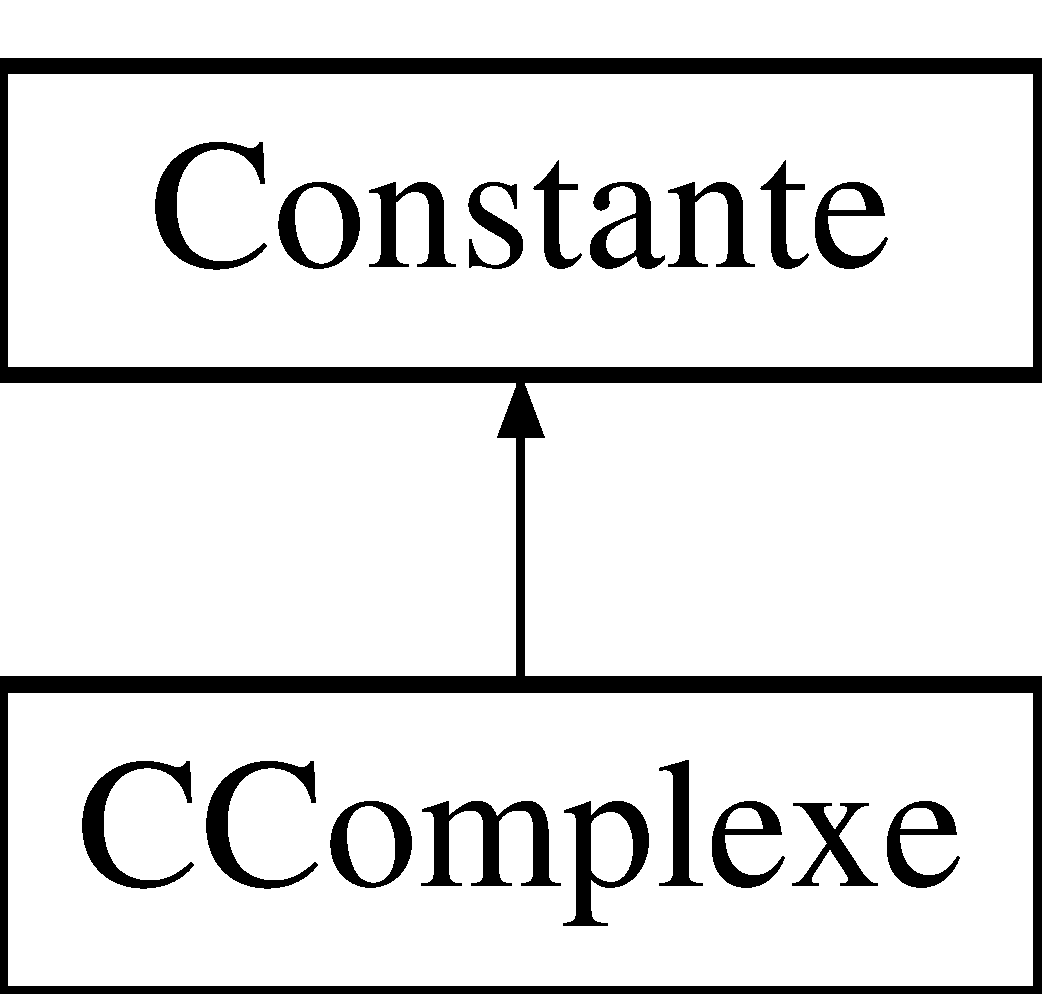
\includegraphics[height=2.000000cm]{class_c_complexe}
\end{center}
\end{figure}
\subsection*{Public Member Functions}
\begin{DoxyCompactItemize}
\item 
\hyperlink{class_c_complexe_afd567f5a10d7fcf6128124b220718973}{C\-Complexe} (\hyperlink{class_constante}{Constante} $\ast$r, \hyperlink{class_constante}{Constante} $\ast$i)
\begin{DoxyCompactList}\small\item\em constructeur. \end{DoxyCompactList}\item 
\hyperlink{class_c_complexe_a20f9638e3ba3600744ec387fa70cc30b}{C\-Complexe} (const \hyperlink{class_c_complexe}{C\-Complexe} \&c)
\begin{DoxyCompactList}\small\item\em constructeur. \end{DoxyCompactList}\item 
\hyperlink{class_constante}{Constante} $\ast$ \hyperlink{class_c_complexe_a5afb89b25938e8c6b457de3b80da5cb0}{get\-Copy} ()
\begin{DoxyCompactList}\small\item\em retourne une copie de la constante \end{DoxyCompactList}\item 
\hypertarget{class_c_complexe_a6dfa179b48b5bb2ba5eb55fec7e971b8}{\hyperlink{class_c_complexe_a6dfa179b48b5bb2ba5eb55fec7e971b8}{$\sim$\-C\-Complexe} ()}\label{class_c_complexe_a6dfa179b48b5bb2ba5eb55fec7e971b8}

\begin{DoxyCompactList}\small\item\em destructeur. \end{DoxyCompactList}\item 
\hyperlink{class_constante}{Constante} $\ast$ \hyperlink{class_c_complexe_a79bf21767456df407987744abc6da88b}{get\-Re} () const 
\begin{DoxyCompactList}\small\item\em retourne la partie reel du complexe. \end{DoxyCompactList}\item 
\hyperlink{class_constante}{Constante} $\ast$ \hyperlink{class_c_complexe_a98d9b7c06bb830be93ab1306a57d716f}{get\-Im} () const 
\begin{DoxyCompactList}\small\item\em retourne la partie imaginaire du complexe. \end{DoxyCompactList}\item 
Q\-String \hyperlink{class_c_complexe_a2ac287ee5fac2c2365fe618f47d235dc}{get\-Valueto\-String} () const 
\begin{DoxyCompactList}\small\item\em retourne le contenu de la constante sous forme de texte \end{DoxyCompactList}\item 
\hyperlink{class_constante}{Constante} $\ast$ \hyperlink{class_c_complexe_a3ff3a06dde38c3fba33fafbef7b3cd99}{operator+} (\hyperlink{class_constante}{Constante} \&c1)
\begin{DoxyCompactList}\small\item\em retourne le resultat de l'operation + entre deux constantes \end{DoxyCompactList}\item 
\hyperlink{class_constante}{Constante} $\ast$ \hyperlink{class_c_complexe_a2661c1f2dedc3f417af1a941f11ca583}{operator-\/} (\hyperlink{class_constante}{Constante} \&c1)
\begin{DoxyCompactList}\small\item\em retourne le resultat de l'operation -\/ entre deux constantes \end{DoxyCompactList}\item 
\hyperlink{class_constante}{Constante} $\ast$ \hyperlink{class_c_complexe_aa0d80726cdd5b1aba17ac25c2bed1194}{operator$\ast$} (\hyperlink{class_constante}{Constante} \&c1)
\begin{DoxyCompactList}\small\item\em retourne le resultat de l'operation $\ast$ entre deux constantes \end{DoxyCompactList}\item 
\hyperlink{class_constante}{Constante} $\ast$ \hyperlink{class_c_complexe_a518ad5669537f64418ef6007687a3297}{operator/} (\hyperlink{class_constante}{Constante} \&c1)
\begin{DoxyCompactList}\small\item\em retourne le resultat de l'operation / entre deux constantes \end{DoxyCompactList}\end{DoxyCompactItemize}


\subsection{Detailed Description}
\hyperlink{class_c_complexe}{C\-Complexe} class. 

classe des types complexes 

\subsection{Constructor \& Destructor Documentation}
\hypertarget{class_c_complexe_afd567f5a10d7fcf6128124b220718973}{\index{C\-Complexe@{C\-Complexe}!C\-Complexe@{C\-Complexe}}
\index{C\-Complexe@{C\-Complexe}!CComplexe@{C\-Complexe}}
\subsubsection[{C\-Complexe}]{\setlength{\rightskip}{0pt plus 5cm}C\-Complexe\-::\-C\-Complexe (
\begin{DoxyParamCaption}
\item[{{\bf Constante} $\ast$}]{r, }
\item[{{\bf Constante} $\ast$}]{i}
\end{DoxyParamCaption}
)\hspace{0.3cm}{\ttfamily [inline]}}}\label{class_c_complexe_afd567f5a10d7fcf6128124b220718973}


constructeur. 


\begin{DoxyParams}{Parameters}
{\em r} & pointeur vers la constante partie reel \\
\hline
{\em i} & pointeur vers la constante partie imaginaire \\
\hline
\end{DoxyParams}
\hypertarget{class_c_complexe_a20f9638e3ba3600744ec387fa70cc30b}{\index{C\-Complexe@{C\-Complexe}!C\-Complexe@{C\-Complexe}}
\index{C\-Complexe@{C\-Complexe}!CComplexe@{C\-Complexe}}
\subsubsection[{C\-Complexe}]{\setlength{\rightskip}{0pt plus 5cm}C\-Complexe\-::\-C\-Complexe (
\begin{DoxyParamCaption}
\item[{const {\bf C\-Complexe} \&}]{c}
\end{DoxyParamCaption}
)\hspace{0.3cm}{\ttfamily [inline]}}}\label{class_c_complexe_a20f9638e3ba3600744ec387fa70cc30b}


constructeur. 


\begin{DoxyParams}{Parameters}
{\em c} & reference vers le \hyperlink{class_c_complexe}{C\-Complexe} a copier \\
\hline
\end{DoxyParams}


\subsection{Member Function Documentation}
\hypertarget{class_c_complexe_a5afb89b25938e8c6b457de3b80da5cb0}{\index{C\-Complexe@{C\-Complexe}!get\-Copy@{get\-Copy}}
\index{get\-Copy@{get\-Copy}!CComplexe@{C\-Complexe}}
\subsubsection[{get\-Copy}]{\setlength{\rightskip}{0pt plus 5cm}{\bf Constante}$\ast$ C\-Complexe\-::get\-Copy (
\begin{DoxyParamCaption}
{}
\end{DoxyParamCaption}
)\hspace{0.3cm}{\ttfamily [inline]}, {\ttfamily [virtual]}}}\label{class_c_complexe_a5afb89b25938e8c6b457de3b80da5cb0}


retourne une copie de la constante 

\begin{DoxyReturn}{Returns}
pointeur vers une copie de la constante 
\end{DoxyReturn}


Implements \hyperlink{class_constante_addd94a5006b4ed68cc0d1d7b5864e10a}{Constante}.

\hypertarget{class_c_complexe_a98d9b7c06bb830be93ab1306a57d716f}{\index{C\-Complexe@{C\-Complexe}!get\-Im@{get\-Im}}
\index{get\-Im@{get\-Im}!CComplexe@{C\-Complexe}}
\subsubsection[{get\-Im}]{\setlength{\rightskip}{0pt plus 5cm}{\bf Constante}$\ast$ C\-Complexe\-::get\-Im (
\begin{DoxyParamCaption}
{}
\end{DoxyParamCaption}
) const\hspace{0.3cm}{\ttfamily [inline]}}}\label{class_c_complexe_a98d9b7c06bb830be93ab1306a57d716f}


retourne la partie imaginaire du complexe. 

\begin{DoxyReturn}{Returns}
pointeur vers la constante partie imaginaire 
\end{DoxyReturn}
\hypertarget{class_c_complexe_a79bf21767456df407987744abc6da88b}{\index{C\-Complexe@{C\-Complexe}!get\-Re@{get\-Re}}
\index{get\-Re@{get\-Re}!CComplexe@{C\-Complexe}}
\subsubsection[{get\-Re}]{\setlength{\rightskip}{0pt plus 5cm}{\bf Constante}$\ast$ C\-Complexe\-::get\-Re (
\begin{DoxyParamCaption}
{}
\end{DoxyParamCaption}
) const\hspace{0.3cm}{\ttfamily [inline]}}}\label{class_c_complexe_a79bf21767456df407987744abc6da88b}


retourne la partie reel du complexe. 

\begin{DoxyReturn}{Returns}
pointeur vers la constante partie reel 
\end{DoxyReturn}
\hypertarget{class_c_complexe_a2ac287ee5fac2c2365fe618f47d235dc}{\index{C\-Complexe@{C\-Complexe}!get\-Valueto\-String@{get\-Valueto\-String}}
\index{get\-Valueto\-String@{get\-Valueto\-String}!CComplexe@{C\-Complexe}}
\subsubsection[{get\-Valueto\-String}]{\setlength{\rightskip}{0pt plus 5cm}Q\-String C\-Complexe\-::get\-Valueto\-String (
\begin{DoxyParamCaption}
{}
\end{DoxyParamCaption}
) const\hspace{0.3cm}{\ttfamily [inline]}, {\ttfamily [virtual]}}}\label{class_c_complexe_a2ac287ee5fac2c2365fe618f47d235dc}


retourne le contenu de la constante sous forme de texte 

\begin{DoxyReturn}{Returns}
Q\-String valeur formatee de la constante 
\end{DoxyReturn}


Implements \hyperlink{class_constante_a93d89080856c972bdebc3619fc957f52}{Constante}.

\hypertarget{class_c_complexe_aa0d80726cdd5b1aba17ac25c2bed1194}{\index{C\-Complexe@{C\-Complexe}!operator$\ast$@{operator$\ast$}}
\index{operator$\ast$@{operator$\ast$}!CComplexe@{C\-Complexe}}
\subsubsection[{operator$\ast$}]{\setlength{\rightskip}{0pt plus 5cm}{\bf Constante} $\ast$ C\-Complexe\-::operator$\ast$ (
\begin{DoxyParamCaption}
\item[{{\bf Constante} \&}]{c1}
\end{DoxyParamCaption}
)\hspace{0.3cm}{\ttfamily [virtual]}}}\label{class_c_complexe_aa0d80726cdd5b1aba17ac25c2bed1194}


retourne le resultat de l'operation $\ast$ entre deux constantes 


\begin{DoxyParams}{Parameters}
{\em c1} & reference vers le deuxieme operande de type \hyperlink{class_constante}{Constante} \\
\hline
\end{DoxyParams}
\begin{DoxyReturn}{Returns}
un pointeur \hyperlink{class_constante}{Constante} sur le resultat 
\end{DoxyReturn}


Implements \hyperlink{class_constante_ae7c4cf6a493277ec98ae346e13bbf82a}{Constante}.

\hypertarget{class_c_complexe_a3ff3a06dde38c3fba33fafbef7b3cd99}{\index{C\-Complexe@{C\-Complexe}!operator+@{operator+}}
\index{operator+@{operator+}!CComplexe@{C\-Complexe}}
\subsubsection[{operator+}]{\setlength{\rightskip}{0pt plus 5cm}{\bf Constante} $\ast$ C\-Complexe\-::operator+ (
\begin{DoxyParamCaption}
\item[{{\bf Constante} \&}]{c1}
\end{DoxyParamCaption}
)\hspace{0.3cm}{\ttfamily [virtual]}}}\label{class_c_complexe_a3ff3a06dde38c3fba33fafbef7b3cd99}


retourne le resultat de l'operation + entre deux constantes 


\begin{DoxyParams}{Parameters}
{\em c1} & reference vers le deuxieme operande de type \hyperlink{class_constante}{Constante} \\
\hline
\end{DoxyParams}
\begin{DoxyReturn}{Returns}
un pointeur \hyperlink{class_constante}{Constante} sur le resultat 
\end{DoxyReturn}


Implements \hyperlink{class_constante_ae1c9e9fa9b3272e37bdb292509741831}{Constante}.

\hypertarget{class_c_complexe_a2661c1f2dedc3f417af1a941f11ca583}{\index{C\-Complexe@{C\-Complexe}!operator-\/@{operator-\/}}
\index{operator-\/@{operator-\/}!CComplexe@{C\-Complexe}}
\subsubsection[{operator-\/}]{\setlength{\rightskip}{0pt plus 5cm}{\bf Constante} $\ast$ C\-Complexe\-::operator-\/ (
\begin{DoxyParamCaption}
\item[{{\bf Constante} \&}]{c1}
\end{DoxyParamCaption}
)\hspace{0.3cm}{\ttfamily [virtual]}}}\label{class_c_complexe_a2661c1f2dedc3f417af1a941f11ca583}


retourne le resultat de l'operation -\/ entre deux constantes 


\begin{DoxyParams}{Parameters}
{\em c1} & reference vers le deuxieme operande de type \hyperlink{class_constante}{Constante} \\
\hline
\end{DoxyParams}
\begin{DoxyReturn}{Returns}
un pointeur \hyperlink{class_constante}{Constante} sur le resultat 
\end{DoxyReturn}


Implements \hyperlink{class_constante_a9d0df3d484c2d87556cb4faa73606862}{Constante}.

\hypertarget{class_c_complexe_a518ad5669537f64418ef6007687a3297}{\index{C\-Complexe@{C\-Complexe}!operator/@{operator/}}
\index{operator/@{operator/}!CComplexe@{C\-Complexe}}
\subsubsection[{operator/}]{\setlength{\rightskip}{0pt plus 5cm}{\bf Constante} $\ast$ C\-Complexe\-::operator/ (
\begin{DoxyParamCaption}
\item[{{\bf Constante} \&}]{c1}
\end{DoxyParamCaption}
)\hspace{0.3cm}{\ttfamily [virtual]}}}\label{class_c_complexe_a518ad5669537f64418ef6007687a3297}


retourne le resultat de l'operation / entre deux constantes 


\begin{DoxyParams}{Parameters}
{\em c1} & reference vers le deuxieme operande de type \hyperlink{class_constante}{Constante} \\
\hline
\end{DoxyParams}
\begin{DoxyReturn}{Returns}
un pointeur \hyperlink{class_constante}{Constante} sur le resultat 
\end{DoxyReturn}


Implements \hyperlink{class_constante_af83c6680a11bc9ca5db49a32864151dd}{Constante}.



The documentation for this class was generated from the following files\-:\begin{DoxyCompactItemize}
\item 
E\-:/\-Dropbox/\-U\-T\-C/\-G\-I02/\-L\-O21/\-Calculatrice/constante.\-h\item 
E\-:/\-Dropbox/\-U\-T\-C/\-G\-I02/\-L\-O21/\-Calculatrice/constante.\-cpp\end{DoxyCompactItemize}

\hypertarget{class_c_entier}{\section{C\-Entier Class Reference}
\label{class_c_entier}\index{C\-Entier@{C\-Entier}}
}


\hyperlink{class_c_entier}{C\-Entier} class.  




{\ttfamily \#include $<$constante.\-h$>$}

Inheritance diagram for C\-Entier\-:\begin{figure}[H]
\begin{center}
\leavevmode
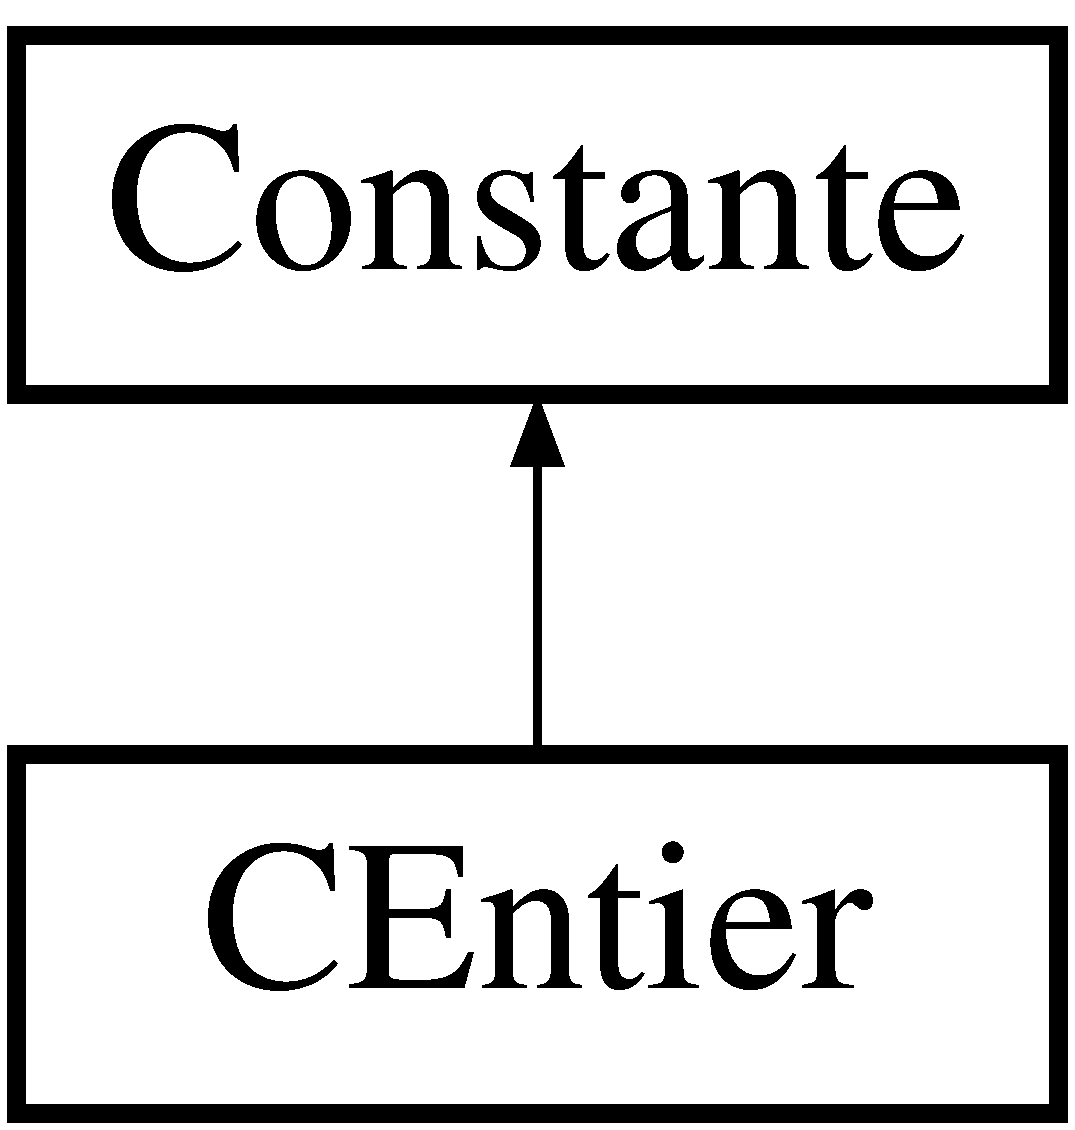
\includegraphics[height=2.000000cm]{class_c_entier}
\end{center}
\end{figure}
\subsection*{Public Member Functions}
\begin{DoxyCompactItemize}
\item 
\hyperlink{class_c_entier_a27467aa3a76b88f836961b7a2536f0f4}{C\-Entier} (int v)
\begin{DoxyCompactList}\small\item\em constructeur. \end{DoxyCompactList}\item 
\hyperlink{class_c_entier_a8374a7a7dc66a7ea59be1fc6cd735376}{C\-Entier} (const \hyperlink{class_c_entier}{C\-Entier} \&c)
\begin{DoxyCompactList}\small\item\em constructeur par copie. \end{DoxyCompactList}\item 
\hyperlink{class_constante}{Constante} $\ast$ \hyperlink{class_c_entier_a48a8a57548157ff88606891b585aa04a}{get\-Copy} ()
\begin{DoxyCompactList}\small\item\em retourne une copie de la constante \end{DoxyCompactList}\item 
int \hyperlink{class_c_entier_a2fcca73095125600ac223a520f5b0ca0}{get\-Value} () const 
\begin{DoxyCompactList}\small\item\em retourne la valeur entier de la constante \end{DoxyCompactList}\item 
void \hyperlink{class_c_entier_a713823920b44ce30efd6c37320c87b93}{set\-Value} (int e)
\begin{DoxyCompactList}\small\item\em affecter une valeur entier a la constante \end{DoxyCompactList}\item 
Q\-String \hyperlink{class_c_entier_ae25f1f0b9422e1d7f256d8e15249e5b6}{get\-Valueto\-String} () const 
\begin{DoxyCompactList}\small\item\em retourne le contenu de la constante sous forme de texte \end{DoxyCompactList}\item 
\hyperlink{class_constante}{Constante} $\ast$ \hyperlink{class_c_entier_a90d87411cff696ada012b426082f9c87}{operator+} (\hyperlink{class_constante}{Constante} \&c1)
\begin{DoxyCompactList}\small\item\em retourne le resultat de l'operation + entre deux constantes \end{DoxyCompactList}\item 
\hyperlink{class_constante}{Constante} $\ast$ \hyperlink{class_c_entier_a5f07b4783dfcfb024cf8c72caac64be7}{operator-\/} (\hyperlink{class_constante}{Constante} \&c1)
\begin{DoxyCompactList}\small\item\em retourne le resultat de l'operation -\/ entre deux constantes \end{DoxyCompactList}\item 
\hyperlink{class_constante}{Constante} $\ast$ \hyperlink{class_c_entier_a2ca548de9fa6c4446d4bd16c0061d3d9}{operator$\ast$} (\hyperlink{class_constante}{Constante} \&c1)
\begin{DoxyCompactList}\small\item\em retourne le resultat de l'operation $\ast$ entre deux constantes \end{DoxyCompactList}\item 
\hyperlink{class_constante}{Constante} $\ast$ \hyperlink{class_c_entier_a0cfb4e65d73cbe8e55be9ade1948d8ec}{operator/} (\hyperlink{class_constante}{Constante} \&c1)
\begin{DoxyCompactList}\small\item\em retourne le resultat de l'operation / entre deux constantes \end{DoxyCompactList}\item 
\hypertarget{class_c_entier_a8a0fdb1aaba3f57969497810665eed33}{\hyperlink{class_c_entier_a8a0fdb1aaba3f57969497810665eed33}{$\sim$\-C\-Entier} ()}\label{class_c_entier_a8a0fdb1aaba3f57969497810665eed33}

\begin{DoxyCompactList}\small\item\em destructeur. \end{DoxyCompactList}\end{DoxyCompactItemize}


\subsection{Detailed Description}
\hyperlink{class_c_entier}{C\-Entier} class. 

classe des types entier 

\subsection{Constructor \& Destructor Documentation}
\hypertarget{class_c_entier_a27467aa3a76b88f836961b7a2536f0f4}{\index{C\-Entier@{C\-Entier}!C\-Entier@{C\-Entier}}
\index{C\-Entier@{C\-Entier}!CEntier@{C\-Entier}}
\subsubsection[{C\-Entier}]{\setlength{\rightskip}{0pt plus 5cm}C\-Entier\-::\-C\-Entier (
\begin{DoxyParamCaption}
\item[{int}]{v}
\end{DoxyParamCaption}
)\hspace{0.3cm}{\ttfamily [inline]}}}\label{class_c_entier_a27467aa3a76b88f836961b7a2536f0f4}


constructeur. 


\begin{DoxyParams}{Parameters}
{\em v} & valeur entiere de la constante \\
\hline
\end{DoxyParams}
\hypertarget{class_c_entier_a8374a7a7dc66a7ea59be1fc6cd735376}{\index{C\-Entier@{C\-Entier}!C\-Entier@{C\-Entier}}
\index{C\-Entier@{C\-Entier}!CEntier@{C\-Entier}}
\subsubsection[{C\-Entier}]{\setlength{\rightskip}{0pt plus 5cm}C\-Entier\-::\-C\-Entier (
\begin{DoxyParamCaption}
\item[{const {\bf C\-Entier} \&}]{c}
\end{DoxyParamCaption}
)\hspace{0.3cm}{\ttfamily [inline]}}}\label{class_c_entier_a8374a7a7dc66a7ea59be1fc6cd735376}


constructeur par copie. 


\begin{DoxyParams}{Parameters}
{\em c} & reference vers la constante a copier \\
\hline
\end{DoxyParams}


\subsection{Member Function Documentation}
\hypertarget{class_c_entier_a48a8a57548157ff88606891b585aa04a}{\index{C\-Entier@{C\-Entier}!get\-Copy@{get\-Copy}}
\index{get\-Copy@{get\-Copy}!CEntier@{C\-Entier}}
\subsubsection[{get\-Copy}]{\setlength{\rightskip}{0pt plus 5cm}{\bf Constante}$\ast$ C\-Entier\-::get\-Copy (
\begin{DoxyParamCaption}
{}
\end{DoxyParamCaption}
)\hspace{0.3cm}{\ttfamily [inline]}, {\ttfamily [virtual]}}}\label{class_c_entier_a48a8a57548157ff88606891b585aa04a}


retourne une copie de la constante 

\begin{DoxyReturn}{Returns}
pointeur vers une copie de la constante 
\end{DoxyReturn}


Implements \hyperlink{class_constante_addd94a5006b4ed68cc0d1d7b5864e10a}{Constante}.

\hypertarget{class_c_entier_a2fcca73095125600ac223a520f5b0ca0}{\index{C\-Entier@{C\-Entier}!get\-Value@{get\-Value}}
\index{get\-Value@{get\-Value}!CEntier@{C\-Entier}}
\subsubsection[{get\-Value}]{\setlength{\rightskip}{0pt plus 5cm}int C\-Entier\-::get\-Value (
\begin{DoxyParamCaption}
{}
\end{DoxyParamCaption}
) const\hspace{0.3cm}{\ttfamily [inline]}}}\label{class_c_entier_a2fcca73095125600ac223a520f5b0ca0}


retourne la valeur entier de la constante 

\begin{DoxyReturn}{Returns}
valeur entiere 
\end{DoxyReturn}
\hypertarget{class_c_entier_ae25f1f0b9422e1d7f256d8e15249e5b6}{\index{C\-Entier@{C\-Entier}!get\-Valueto\-String@{get\-Valueto\-String}}
\index{get\-Valueto\-String@{get\-Valueto\-String}!CEntier@{C\-Entier}}
\subsubsection[{get\-Valueto\-String}]{\setlength{\rightskip}{0pt plus 5cm}Q\-String C\-Entier\-::get\-Valueto\-String (
\begin{DoxyParamCaption}
{}
\end{DoxyParamCaption}
) const\hspace{0.3cm}{\ttfamily [inline]}, {\ttfamily [virtual]}}}\label{class_c_entier_ae25f1f0b9422e1d7f256d8e15249e5b6}


retourne le contenu de la constante sous forme de texte 

\begin{DoxyReturn}{Returns}
Q\-String valeur formatee de la constante 
\end{DoxyReturn}


Implements \hyperlink{class_constante_a93d89080856c972bdebc3619fc957f52}{Constante}.

\hypertarget{class_c_entier_a2ca548de9fa6c4446d4bd16c0061d3d9}{\index{C\-Entier@{C\-Entier}!operator$\ast$@{operator$\ast$}}
\index{operator$\ast$@{operator$\ast$}!CEntier@{C\-Entier}}
\subsubsection[{operator$\ast$}]{\setlength{\rightskip}{0pt plus 5cm}{\bf Constante} $\ast$ C\-Entier\-::operator$\ast$ (
\begin{DoxyParamCaption}
\item[{{\bf Constante} \&}]{c1}
\end{DoxyParamCaption}
)\hspace{0.3cm}{\ttfamily [virtual]}}}\label{class_c_entier_a2ca548de9fa6c4446d4bd16c0061d3d9}


retourne le resultat de l'operation $\ast$ entre deux constantes 


\begin{DoxyParams}{Parameters}
{\em c1} & reference vers le deuxieme operande de type \hyperlink{class_constante}{Constante} \\
\hline
\end{DoxyParams}
\begin{DoxyReturn}{Returns}
un pointeur \hyperlink{class_constante}{Constante} sur le resultat 
\end{DoxyReturn}


Implements \hyperlink{class_constante_ae7c4cf6a493277ec98ae346e13bbf82a}{Constante}.

\hypertarget{class_c_entier_a90d87411cff696ada012b426082f9c87}{\index{C\-Entier@{C\-Entier}!operator+@{operator+}}
\index{operator+@{operator+}!CEntier@{C\-Entier}}
\subsubsection[{operator+}]{\setlength{\rightskip}{0pt plus 5cm}{\bf Constante} $\ast$ C\-Entier\-::operator+ (
\begin{DoxyParamCaption}
\item[{{\bf Constante} \&}]{c1}
\end{DoxyParamCaption}
)\hspace{0.3cm}{\ttfamily [virtual]}}}\label{class_c_entier_a90d87411cff696ada012b426082f9c87}


retourne le resultat de l'operation + entre deux constantes 


\begin{DoxyParams}{Parameters}
{\em c1} & reference vers le deuxieme operande de type \hyperlink{class_constante}{Constante} \\
\hline
\end{DoxyParams}
\begin{DoxyReturn}{Returns}
un pointeur \hyperlink{class_constante}{Constante} sur le resultat 
\end{DoxyReturn}


Implements \hyperlink{class_constante_ae1c9e9fa9b3272e37bdb292509741831}{Constante}.

\hypertarget{class_c_entier_a5f07b4783dfcfb024cf8c72caac64be7}{\index{C\-Entier@{C\-Entier}!operator-\/@{operator-\/}}
\index{operator-\/@{operator-\/}!CEntier@{C\-Entier}}
\subsubsection[{operator-\/}]{\setlength{\rightskip}{0pt plus 5cm}{\bf Constante} $\ast$ C\-Entier\-::operator-\/ (
\begin{DoxyParamCaption}
\item[{{\bf Constante} \&}]{c1}
\end{DoxyParamCaption}
)\hspace{0.3cm}{\ttfamily [virtual]}}}\label{class_c_entier_a5f07b4783dfcfb024cf8c72caac64be7}


retourne le resultat de l'operation -\/ entre deux constantes 


\begin{DoxyParams}{Parameters}
{\em c1} & reference vers le deuxieme operande de type \hyperlink{class_constante}{Constante} \\
\hline
\end{DoxyParams}
\begin{DoxyReturn}{Returns}
un pointeur \hyperlink{class_constante}{Constante} sur le resultat 
\end{DoxyReturn}


Implements \hyperlink{class_constante_a9d0df3d484c2d87556cb4faa73606862}{Constante}.

\hypertarget{class_c_entier_a0cfb4e65d73cbe8e55be9ade1948d8ec}{\index{C\-Entier@{C\-Entier}!operator/@{operator/}}
\index{operator/@{operator/}!CEntier@{C\-Entier}}
\subsubsection[{operator/}]{\setlength{\rightskip}{0pt plus 5cm}{\bf Constante} $\ast$ C\-Entier\-::operator/ (
\begin{DoxyParamCaption}
\item[{{\bf Constante} \&}]{c1}
\end{DoxyParamCaption}
)\hspace{0.3cm}{\ttfamily [virtual]}}}\label{class_c_entier_a0cfb4e65d73cbe8e55be9ade1948d8ec}


retourne le resultat de l'operation / entre deux constantes 


\begin{DoxyParams}{Parameters}
{\em c1} & reference vers le deuxieme operande de type \hyperlink{class_constante}{Constante} \\
\hline
\end{DoxyParams}
\begin{DoxyReturn}{Returns}
un pointeur \hyperlink{class_constante}{Constante} sur le resultat 
\end{DoxyReturn}


Implements \hyperlink{class_constante_af83c6680a11bc9ca5db49a32864151dd}{Constante}.

\hypertarget{class_c_entier_a713823920b44ce30efd6c37320c87b93}{\index{C\-Entier@{C\-Entier}!set\-Value@{set\-Value}}
\index{set\-Value@{set\-Value}!CEntier@{C\-Entier}}
\subsubsection[{set\-Value}]{\setlength{\rightskip}{0pt plus 5cm}void C\-Entier\-::set\-Value (
\begin{DoxyParamCaption}
\item[{int}]{e}
\end{DoxyParamCaption}
)\hspace{0.3cm}{\ttfamily [inline]}}}\label{class_c_entier_a713823920b44ce30efd6c37320c87b93}


affecter une valeur entier a la constante 


\begin{DoxyParams}{Parameters}
{\em e} & valeur entiere \\
\hline
\end{DoxyParams}


The documentation for this class was generated from the following files\-:\begin{DoxyCompactItemize}
\item 
E\-:/\-Dropbox/\-U\-T\-C/\-G\-I02/\-L\-O21/\-Calculatrice/constante.\-h\item 
E\-:/\-Dropbox/\-U\-T\-C/\-G\-I02/\-L\-O21/\-Calculatrice/constante.\-cpp\end{DoxyCompactItemize}

\hypertarget{class_c_expression}{\section{C\-Expression Class Reference}
\label{class_c_expression}\index{C\-Expression@{C\-Expression}}
}


\hyperlink{class_c_expression}{C\-Expression} class.  




{\ttfamily \#include $<$constante.\-h$>$}

Inheritance diagram for C\-Expression\-:\begin{figure}[H]
\begin{center}
\leavevmode
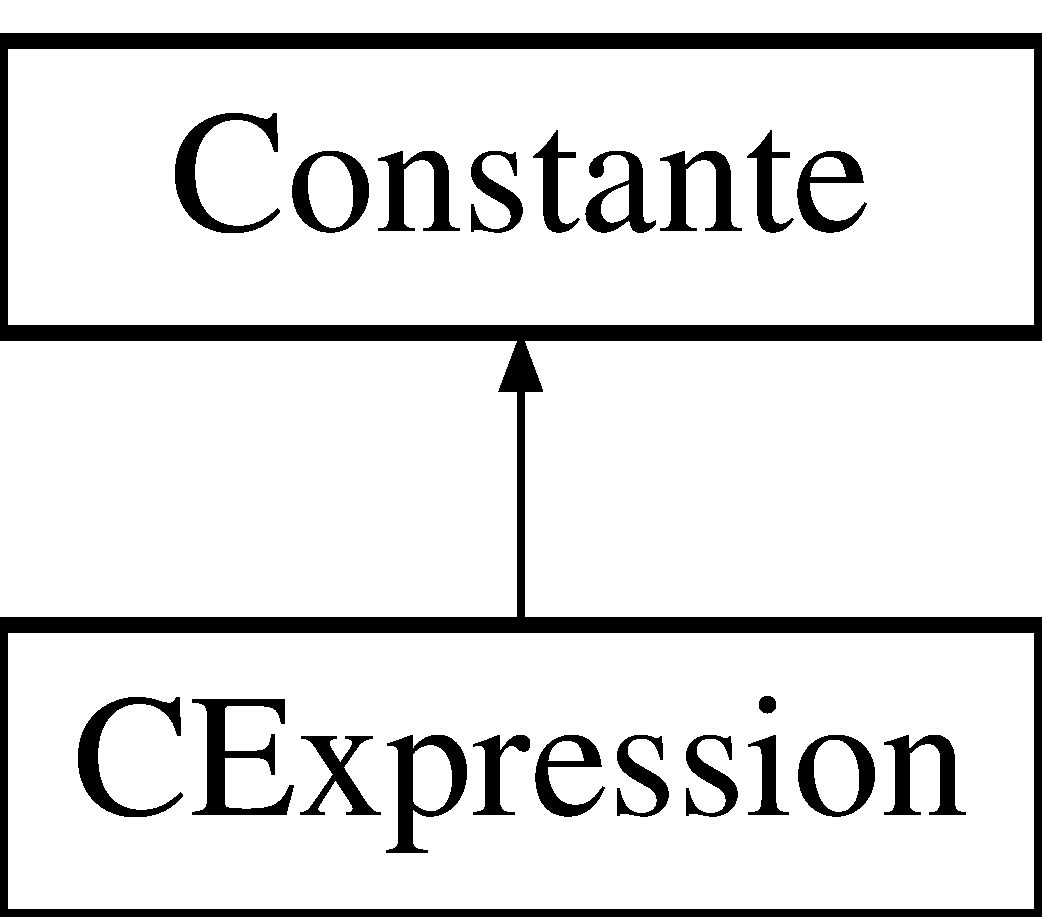
\includegraphics[height=2.000000cm]{class_c_expression}
\end{center}
\end{figure}
\subsection*{Public Member Functions}
\begin{DoxyCompactItemize}
\item 
\hyperlink{class_c_expression_abe2a95c195c0f029e043713e6b2bd9b4}{C\-Expression} (const Q\-String \&ex)
\begin{DoxyCompactList}\small\item\em constructeur. \end{DoxyCompactList}\item 
\hyperlink{class_c_expression_aaf547abee194320f2c2edcb537f35bb3}{C\-Expression} (const \hyperlink{class_c_expression}{C\-Expression} \&c)
\begin{DoxyCompactList}\small\item\em constructeur par copie. \end{DoxyCompactList}\item 
\hyperlink{class_constante}{Constante} $\ast$ \hyperlink{class_c_expression_a0fbadaea165e135c3e12bc35b31a2d55}{get\-Copy} ()
\begin{DoxyCompactList}\small\item\em retourne une copie de la constante \end{DoxyCompactList}\item 
Q\-String \hyperlink{class_c_expression_a54a798d90fe842c6e95f2c85fc73e0f6}{get\-Exp} () const 
\begin{DoxyCompactList}\small\item\em retourne la valeur de l'expression \end{DoxyCompactList}\item 
void \hyperlink{class_c_expression_adcac8fc467b9eeedcba5f5eab4e390b6}{set\-Exp} (const Q\-String \&e)
\begin{DoxyCompactList}\small\item\em affecte l'expression \end{DoxyCompactList}\item 
Q\-String \hyperlink{class_c_expression_a642f89de974553f82cff731f6d83fea6}{get\-Valueto\-String} () const 
\begin{DoxyCompactList}\small\item\em retourne le contenu de la constante sous forme de texte \end{DoxyCompactList}\item 
\hyperlink{class_constante}{Constante} $\ast$ \hyperlink{class_c_expression_acd13043bccbe2e9d63604ecc9b1b2917}{operator-\/} (Q\-String e)
\begin{DoxyCompactList}\small\item\em effectue l'operation -\/ inversee \end{DoxyCompactList}\item 
\hyperlink{class_constante}{Constante} $\ast$ \hyperlink{class_c_expression_af5816c2cd38da72d65631f1b8f7c67e8}{operator/} (Q\-String e)
\begin{DoxyCompactList}\small\item\em affectue l'operation / inversee \end{DoxyCompactList}\item 
\hyperlink{class_constante}{Constante} $\ast$ \hyperlink{class_c_expression_a673be1d66195b8ee7fac79b53d8cf371}{operator+} (\hyperlink{class_constante}{Constante} \&c1)
\begin{DoxyCompactList}\small\item\em retourne le resultat de l'operation + entre deux constantes \end{DoxyCompactList}\item 
\hyperlink{class_constante}{Constante} $\ast$ \hyperlink{class_c_expression_af7fdc3e9fa28257c0cdfed04995cbe8e}{operator-\/} (\hyperlink{class_constante}{Constante} \&c1)
\begin{DoxyCompactList}\small\item\em retourne le resultat de l'operation -\/ entre deux constantes \end{DoxyCompactList}\item 
\hyperlink{class_constante}{Constante} $\ast$ \hyperlink{class_c_expression_a0bcd0e43fe294b187d7ff7240a246ac2}{operator$\ast$} (\hyperlink{class_constante}{Constante} \&c1)
\begin{DoxyCompactList}\small\item\em retourne le resultat de l'operation $\ast$ entre deux constantes \end{DoxyCompactList}\item 
\hyperlink{class_constante}{Constante} $\ast$ \hyperlink{class_c_expression_a92584ee17ad2f42488a37aa991fa3352}{operator/} (\hyperlink{class_constante}{Constante} \&c1)
\begin{DoxyCompactList}\small\item\em retourne le resultat de l'operation / entre deux constantes \end{DoxyCompactList}\item 
\hypertarget{class_c_expression_a622d1164b24e06c6393ea8c2eb387fb0}{\hyperlink{class_c_expression_a622d1164b24e06c6393ea8c2eb387fb0}{$\sim$\-C\-Expression} ()}\label{class_c_expression_a622d1164b24e06c6393ea8c2eb387fb0}

\begin{DoxyCompactList}\small\item\em destructeur. \end{DoxyCompactList}\end{DoxyCompactItemize}


\subsection{Detailed Description}
\hyperlink{class_c_expression}{C\-Expression} class. 

classe des types expressions 

\subsection{Constructor \& Destructor Documentation}
\hypertarget{class_c_expression_abe2a95c195c0f029e043713e6b2bd9b4}{\index{C\-Expression@{C\-Expression}!C\-Expression@{C\-Expression}}
\index{C\-Expression@{C\-Expression}!CExpression@{C\-Expression}}
\subsubsection[{C\-Expression}]{\setlength{\rightskip}{0pt plus 5cm}C\-Expression\-::\-C\-Expression (
\begin{DoxyParamCaption}
\item[{const Q\-String \&}]{ex}
\end{DoxyParamCaption}
)\hspace{0.3cm}{\ttfamily [inline]}}}\label{class_c_expression_abe2a95c195c0f029e043713e6b2bd9b4}


constructeur. 


\begin{DoxyParams}{Parameters}
{\em ex} & expression \\
\hline
\end{DoxyParams}
\hypertarget{class_c_expression_aaf547abee194320f2c2edcb537f35bb3}{\index{C\-Expression@{C\-Expression}!C\-Expression@{C\-Expression}}
\index{C\-Expression@{C\-Expression}!CExpression@{C\-Expression}}
\subsubsection[{C\-Expression}]{\setlength{\rightskip}{0pt plus 5cm}C\-Expression\-::\-C\-Expression (
\begin{DoxyParamCaption}
\item[{const {\bf C\-Expression} \&}]{c}
\end{DoxyParamCaption}
)\hspace{0.3cm}{\ttfamily [inline]}}}\label{class_c_expression_aaf547abee194320f2c2edcb537f35bb3}


constructeur par copie. 


\begin{DoxyParams}{Parameters}
{\em c} & reference de l'expression a copier \\
\hline
\end{DoxyParams}


\subsection{Member Function Documentation}
\hypertarget{class_c_expression_a0fbadaea165e135c3e12bc35b31a2d55}{\index{C\-Expression@{C\-Expression}!get\-Copy@{get\-Copy}}
\index{get\-Copy@{get\-Copy}!CExpression@{C\-Expression}}
\subsubsection[{get\-Copy}]{\setlength{\rightskip}{0pt plus 5cm}{\bf Constante}$\ast$ C\-Expression\-::get\-Copy (
\begin{DoxyParamCaption}
{}
\end{DoxyParamCaption}
)\hspace{0.3cm}{\ttfamily [inline]}, {\ttfamily [virtual]}}}\label{class_c_expression_a0fbadaea165e135c3e12bc35b31a2d55}


retourne une copie de la constante 

\begin{DoxyReturn}{Returns}
pointeur vers une copie de la constante 
\end{DoxyReturn}


Implements \hyperlink{class_constante_addd94a5006b4ed68cc0d1d7b5864e10a}{Constante}.

\hypertarget{class_c_expression_a54a798d90fe842c6e95f2c85fc73e0f6}{\index{C\-Expression@{C\-Expression}!get\-Exp@{get\-Exp}}
\index{get\-Exp@{get\-Exp}!CExpression@{C\-Expression}}
\subsubsection[{get\-Exp}]{\setlength{\rightskip}{0pt plus 5cm}Q\-String C\-Expression\-::get\-Exp (
\begin{DoxyParamCaption}
{}
\end{DoxyParamCaption}
) const\hspace{0.3cm}{\ttfamily [inline]}}}\label{class_c_expression_a54a798d90fe842c6e95f2c85fc73e0f6}


retourne la valeur de l'expression 

\begin{DoxyReturn}{Returns}
Q\-String expression 
\end{DoxyReturn}
\hypertarget{class_c_expression_a642f89de974553f82cff731f6d83fea6}{\index{C\-Expression@{C\-Expression}!get\-Valueto\-String@{get\-Valueto\-String}}
\index{get\-Valueto\-String@{get\-Valueto\-String}!CExpression@{C\-Expression}}
\subsubsection[{get\-Valueto\-String}]{\setlength{\rightskip}{0pt plus 5cm}Q\-String C\-Expression\-::get\-Valueto\-String (
\begin{DoxyParamCaption}
{}
\end{DoxyParamCaption}
) const\hspace{0.3cm}{\ttfamily [inline]}, {\ttfamily [virtual]}}}\label{class_c_expression_a642f89de974553f82cff731f6d83fea6}


retourne le contenu de la constante sous forme de texte 

\begin{DoxyReturn}{Returns}
Q\-String valeur formatee de la constante 
\end{DoxyReturn}


Implements \hyperlink{class_constante_a93d89080856c972bdebc3619fc957f52}{Constante}.

\hypertarget{class_c_expression_a0bcd0e43fe294b187d7ff7240a246ac2}{\index{C\-Expression@{C\-Expression}!operator$\ast$@{operator$\ast$}}
\index{operator$\ast$@{operator$\ast$}!CExpression@{C\-Expression}}
\subsubsection[{operator$\ast$}]{\setlength{\rightskip}{0pt plus 5cm}{\bf Constante} $\ast$ C\-Expression\-::operator$\ast$ (
\begin{DoxyParamCaption}
\item[{{\bf Constante} \&}]{c1}
\end{DoxyParamCaption}
)\hspace{0.3cm}{\ttfamily [virtual]}}}\label{class_c_expression_a0bcd0e43fe294b187d7ff7240a246ac2}


retourne le resultat de l'operation $\ast$ entre deux constantes 


\begin{DoxyParams}{Parameters}
{\em c1} & reference vers le deuxieme operande de type \hyperlink{class_constante}{Constante} \\
\hline
\end{DoxyParams}
\begin{DoxyReturn}{Returns}
un pointeur \hyperlink{class_constante}{Constante} sur le resultat 
\end{DoxyReturn}


Implements \hyperlink{class_constante_ae7c4cf6a493277ec98ae346e13bbf82a}{Constante}.

\hypertarget{class_c_expression_a673be1d66195b8ee7fac79b53d8cf371}{\index{C\-Expression@{C\-Expression}!operator+@{operator+}}
\index{operator+@{operator+}!CExpression@{C\-Expression}}
\subsubsection[{operator+}]{\setlength{\rightskip}{0pt plus 5cm}{\bf Constante} $\ast$ C\-Expression\-::operator+ (
\begin{DoxyParamCaption}
\item[{{\bf Constante} \&}]{c1}
\end{DoxyParamCaption}
)\hspace{0.3cm}{\ttfamily [virtual]}}}\label{class_c_expression_a673be1d66195b8ee7fac79b53d8cf371}


retourne le resultat de l'operation + entre deux constantes 


\begin{DoxyParams}{Parameters}
{\em c1} & reference vers le deuxieme operande de type \hyperlink{class_constante}{Constante} \\
\hline
\end{DoxyParams}
\begin{DoxyReturn}{Returns}
un pointeur \hyperlink{class_constante}{Constante} sur le resultat 
\end{DoxyReturn}


Implements \hyperlink{class_constante_ae1c9e9fa9b3272e37bdb292509741831}{Constante}.

\hypertarget{class_c_expression_acd13043bccbe2e9d63604ecc9b1b2917}{\index{C\-Expression@{C\-Expression}!operator-\/@{operator-\/}}
\index{operator-\/@{operator-\/}!CExpression@{C\-Expression}}
\subsubsection[{operator-\/}]{\setlength{\rightskip}{0pt plus 5cm}{\bf Constante} $\ast$ C\-Expression\-::operator-\/ (
\begin{DoxyParamCaption}
\item[{Q\-String}]{e}
\end{DoxyParamCaption}
)}}\label{class_c_expression_acd13043bccbe2e9d63604ecc9b1b2917}


effectue l'operation -\/ inversee 


\begin{DoxyParams}{Parameters}
{\em e} & valeur a ajouter \\
\hline
\end{DoxyParams}
\hypertarget{class_c_expression_af7fdc3e9fa28257c0cdfed04995cbe8e}{\index{C\-Expression@{C\-Expression}!operator-\/@{operator-\/}}
\index{operator-\/@{operator-\/}!CExpression@{C\-Expression}}
\subsubsection[{operator-\/}]{\setlength{\rightskip}{0pt plus 5cm}{\bf Constante} $\ast$ C\-Expression\-::operator-\/ (
\begin{DoxyParamCaption}
\item[{{\bf Constante} \&}]{c1}
\end{DoxyParamCaption}
)\hspace{0.3cm}{\ttfamily [virtual]}}}\label{class_c_expression_af7fdc3e9fa28257c0cdfed04995cbe8e}


retourne le resultat de l'operation -\/ entre deux constantes 


\begin{DoxyParams}{Parameters}
{\em c1} & reference vers le deuxieme operande de type \hyperlink{class_constante}{Constante} \\
\hline
\end{DoxyParams}
\begin{DoxyReturn}{Returns}
un pointeur \hyperlink{class_constante}{Constante} sur le resultat 
\end{DoxyReturn}


Implements \hyperlink{class_constante_a9d0df3d484c2d87556cb4faa73606862}{Constante}.

\hypertarget{class_c_expression_af5816c2cd38da72d65631f1b8f7c67e8}{\index{C\-Expression@{C\-Expression}!operator/@{operator/}}
\index{operator/@{operator/}!CExpression@{C\-Expression}}
\subsubsection[{operator/}]{\setlength{\rightskip}{0pt plus 5cm}{\bf Constante} $\ast$ C\-Expression\-::operator/ (
\begin{DoxyParamCaption}
\item[{Q\-String}]{e}
\end{DoxyParamCaption}
)}}\label{class_c_expression_af5816c2cd38da72d65631f1b8f7c67e8}


affectue l'operation / inversee 


\begin{DoxyParams}{Parameters}
{\em e} & valeur a ajouter \\
\hline
\end{DoxyParams}
\hypertarget{class_c_expression_a92584ee17ad2f42488a37aa991fa3352}{\index{C\-Expression@{C\-Expression}!operator/@{operator/}}
\index{operator/@{operator/}!CExpression@{C\-Expression}}
\subsubsection[{operator/}]{\setlength{\rightskip}{0pt plus 5cm}{\bf Constante} $\ast$ C\-Expression\-::operator/ (
\begin{DoxyParamCaption}
\item[{{\bf Constante} \&}]{c1}
\end{DoxyParamCaption}
)\hspace{0.3cm}{\ttfamily [virtual]}}}\label{class_c_expression_a92584ee17ad2f42488a37aa991fa3352}


retourne le resultat de l'operation / entre deux constantes 


\begin{DoxyParams}{Parameters}
{\em c1} & reference vers le deuxieme operande de type \hyperlink{class_constante}{Constante} \\
\hline
\end{DoxyParams}
\begin{DoxyReturn}{Returns}
un pointeur \hyperlink{class_constante}{Constante} sur le resultat 
\end{DoxyReturn}


Implements \hyperlink{class_constante_af83c6680a11bc9ca5db49a32864151dd}{Constante}.

\hypertarget{class_c_expression_adcac8fc467b9eeedcba5f5eab4e390b6}{\index{C\-Expression@{C\-Expression}!set\-Exp@{set\-Exp}}
\index{set\-Exp@{set\-Exp}!CExpression@{C\-Expression}}
\subsubsection[{set\-Exp}]{\setlength{\rightskip}{0pt plus 5cm}void C\-Expression\-::set\-Exp (
\begin{DoxyParamCaption}
\item[{const Q\-String \&}]{e}
\end{DoxyParamCaption}
)\hspace{0.3cm}{\ttfamily [inline]}}}\label{class_c_expression_adcac8fc467b9eeedcba5f5eab4e390b6}


affecte l'expression 


\begin{DoxyParams}{Parameters}
{\em e} & expression \\
\hline
\end{DoxyParams}


The documentation for this class was generated from the following files\-:\begin{DoxyCompactItemize}
\item 
E\-:/\-Dropbox/\-U\-T\-C/\-G\-I02/\-L\-O21/\-Calculatrice/constante.\-h\item 
E\-:/\-Dropbox/\-U\-T\-C/\-G\-I02/\-L\-O21/\-Calculatrice/constante.\-cpp\end{DoxyCompactItemize}

\hypertarget{class_commande}{\section{Commande Class Reference}
\label{class_commande}\index{Commande@{Commande}}
}


\hyperlink{class_commande}{Commande} class.  




{\ttfamily \#include $<$commande.\-h$>$}

Inheritance diagram for Commande\-:\begin{figure}[H]
\begin{center}
\leavevmode
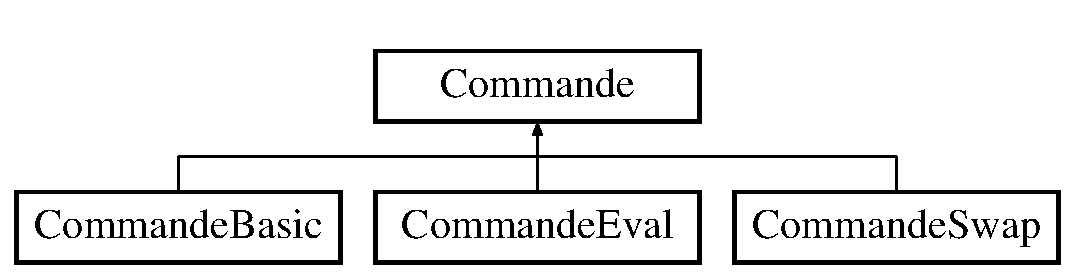
\includegraphics[height=2.000000cm]{class_commande}
\end{center}
\end{figure}
\subsection*{Public Member Functions}
\begin{DoxyCompactItemize}
\item 
\hypertarget{class_commande_a9fc0c740359ac4f0d34b9f109e3c0155}{virtual void \hyperlink{class_commande_a9fc0c740359ac4f0d34b9f109e3c0155}{Do} ()=0}\label{class_commande_a9fc0c740359ac4f0d34b9f109e3c0155}

\begin{DoxyCompactList}\small\item\em executer l'operation \end{DoxyCompactList}\item 
\hypertarget{class_commande_a8523106c6ca6cc7c04323a641c16e563}{virtual void \hyperlink{class_commande_a8523106c6ca6cc7c04323a641c16e563}{Undo} ()=0}\label{class_commande_a8523106c6ca6cc7c04323a641c16e563}

\begin{DoxyCompactList}\small\item\em executer l'operation inverse \end{DoxyCompactList}\item 
\hypertarget{class_commande_ad2c20aed07bfd27f220daf3dc316bbb5}{virtual void \hyperlink{class_commande_ad2c20aed07bfd27f220daf3dc316bbb5}{Vider} ()=0}\label{class_commande_ad2c20aed07bfd27f220daf3dc316bbb5}

\begin{DoxyCompactList}\small\item\em vide les piles de la commande. \end{DoxyCompactList}\end{DoxyCompactItemize}


\subsection{Detailed Description}
\hyperlink{class_commande}{Commande} class. 

classe virtuelle des commandes 

The documentation for this class was generated from the following file\-:\begin{DoxyCompactItemize}
\item 
E\-:/\-Dropbox/\-U\-T\-C/\-G\-I02/\-L\-O21/\-Calculatrice/commande.\-h\end{DoxyCompactItemize}

\hypertarget{class_commande_basic}{\section{Commande\-Basic Class Reference}
\label{class_commande_basic}\index{Commande\-Basic@{Commande\-Basic}}
}


\hyperlink{class_commande_basic}{Commande\-Basic} class.  




{\ttfamily \#include $<$commande.\-h$>$}

Inheritance diagram for Commande\-Basic\-:\begin{figure}[H]
\begin{center}
\leavevmode
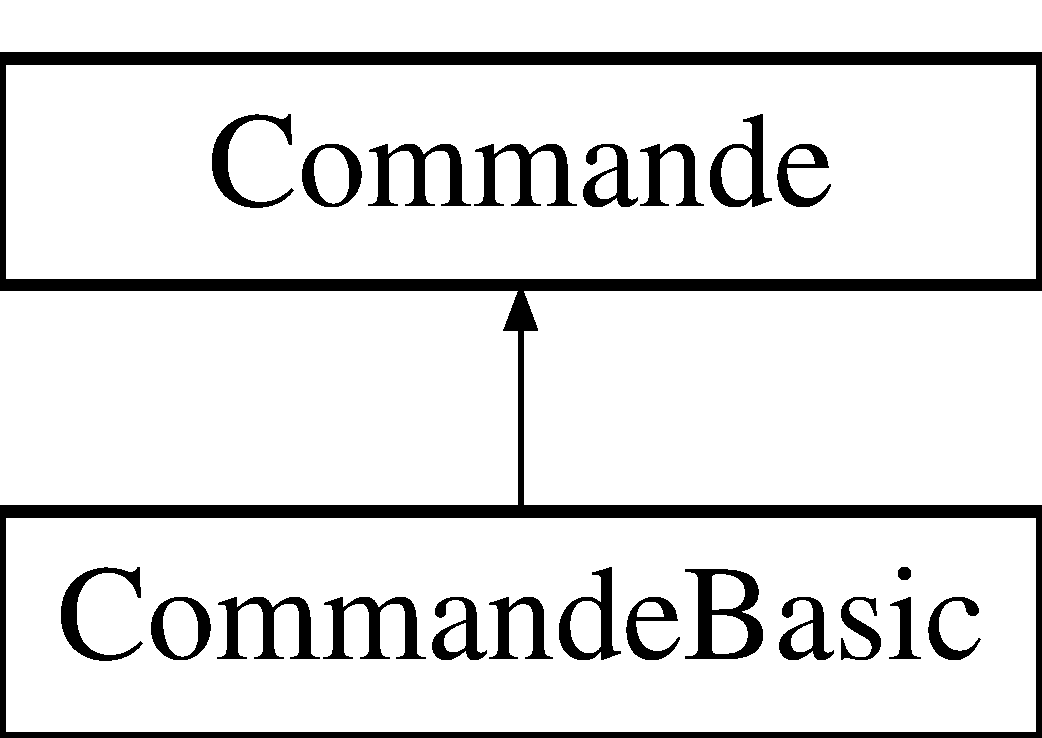
\includegraphics[height=2.000000cm]{class_commande_basic}
\end{center}
\end{figure}
\subsection*{Public Member Functions}
\begin{DoxyCompactItemize}
\item 
\hyperlink{class_commande_basic_a06896fb033075c9ad816cdc054cffa7c}{Commande\-Basic} (\hyperlink{class_pile}{Pile} $\ast$p)
\begin{DoxyCompactList}\small\item\em constructeur. \end{DoxyCompactList}\item 
\hyperlink{class_commande_basic_a0e14f93e2dac91cf302ab1eeefd72efc}{$\sim$\-Commande\-Basic} ()
\begin{DoxyCompactList}\small\item\em destructeur. \end{DoxyCompactList}\item 
\hypertarget{class_commande_basic_ad249aebd20fc1e2971daa3c1b915920c}{void \hyperlink{class_commande_basic_ad249aebd20fc1e2971daa3c1b915920c}{Vider} ()}\label{class_commande_basic_ad249aebd20fc1e2971daa3c1b915920c}

\begin{DoxyCompactList}\small\item\em vide les piles de la commande. \end{DoxyCompactList}\item 
void \hyperlink{class_commande_basic_aee8cf6044f00f87f26995ab28bfa5e91}{add\-Old} (\hyperlink{class_constante}{Constante} $\ast$c)
\begin{DoxyCompactList}\small\item\em ajoute une constante a la pile old\-Const. \end{DoxyCompactList}\item 
void \hyperlink{class_commande_basic_aedeb00c48e9990847cf54753acb93d7e}{add\-New} (\hyperlink{class_constante}{Constante} $\ast$c)
\begin{DoxyCompactList}\small\item\em ajoute une constante a la pile new\-Const. \end{DoxyCompactList}\item 
void \hyperlink{class_commande_basic_a1a0e1350aa80995f26dec83e56cb27e7}{Do} ()
\begin{DoxyCompactList}\small\item\em executer l'operation \end{DoxyCompactList}\item 
void \hyperlink{class_commande_basic_ab5c5afa269142fc2aa49987b7ae31601}{Undo} ()
\begin{DoxyCompactList}\small\item\em executer l'operation inverse \end{DoxyCompactList}\end{DoxyCompactItemize}


\subsection{Detailed Description}
\hyperlink{class_commande_basic}{Commande\-Basic} class. 

traite la majorite des commandes de la calculatrice. 

\subsection{Constructor \& Destructor Documentation}
\hypertarget{class_commande_basic_a06896fb033075c9ad816cdc054cffa7c}{\index{Commande\-Basic@{Commande\-Basic}!Commande\-Basic@{Commande\-Basic}}
\index{Commande\-Basic@{Commande\-Basic}!CommandeBasic@{Commande\-Basic}}
\subsubsection[{Commande\-Basic}]{\setlength{\rightskip}{0pt plus 5cm}Commande\-Basic\-::\-Commande\-Basic (
\begin{DoxyParamCaption}
\item[{{\bf Pile} $\ast$}]{p}
\end{DoxyParamCaption}
)\hspace{0.3cm}{\ttfamily [inline]}}}\label{class_commande_basic_a06896fb033075c9ad816cdc054cffa7c}


constructeur. 


\begin{DoxyParams}{Parameters}
{\em p} & Pointeur vers la pile stockant la commande \\
\hline
\end{DoxyParams}
\hypertarget{class_commande_basic_a0e14f93e2dac91cf302ab1eeefd72efc}{\index{Commande\-Basic@{Commande\-Basic}!$\sim$\-Commande\-Basic@{$\sim$\-Commande\-Basic}}
\index{$\sim$\-Commande\-Basic@{$\sim$\-Commande\-Basic}!CommandeBasic@{Commande\-Basic}}
\subsubsection[{$\sim$\-Commande\-Basic}]{\setlength{\rightskip}{0pt plus 5cm}Commande\-Basic\-::$\sim$\-Commande\-Basic (
\begin{DoxyParamCaption}
{}
\end{DoxyParamCaption}
)}}\label{class_commande_basic_a0e14f93e2dac91cf302ab1eeefd72efc}


destructeur. 

detruit la commande et les constantes de la pile new\-Const 

\subsection{Member Function Documentation}
\hypertarget{class_commande_basic_aedeb00c48e9990847cf54753acb93d7e}{\index{Commande\-Basic@{Commande\-Basic}!add\-New@{add\-New}}
\index{add\-New@{add\-New}!CommandeBasic@{Commande\-Basic}}
\subsubsection[{add\-New}]{\setlength{\rightskip}{0pt plus 5cm}void Commande\-Basic\-::add\-New (
\begin{DoxyParamCaption}
\item[{{\bf Constante} $\ast$}]{c}
\end{DoxyParamCaption}
)}}\label{class_commande_basic_aedeb00c48e9990847cf54753acb93d7e}


ajoute une constante a la pile new\-Const. 


\begin{DoxyParams}{Parameters}
{\em c} & Pointeur vers la constante a stocker \\
\hline
\end{DoxyParams}
\hypertarget{class_commande_basic_aee8cf6044f00f87f26995ab28bfa5e91}{\index{Commande\-Basic@{Commande\-Basic}!add\-Old@{add\-Old}}
\index{add\-Old@{add\-Old}!CommandeBasic@{Commande\-Basic}}
\subsubsection[{add\-Old}]{\setlength{\rightskip}{0pt plus 5cm}void Commande\-Basic\-::add\-Old (
\begin{DoxyParamCaption}
\item[{{\bf Constante} $\ast$}]{c}
\end{DoxyParamCaption}
)}}\label{class_commande_basic_aee8cf6044f00f87f26995ab28bfa5e91}


ajoute une constante a la pile old\-Const. 


\begin{DoxyParams}{Parameters}
{\em c} & Pointeur vers la constante a stocker \\
\hline
\end{DoxyParams}
\hypertarget{class_commande_basic_a1a0e1350aa80995f26dec83e56cb27e7}{\index{Commande\-Basic@{Commande\-Basic}!Do@{Do}}
\index{Do@{Do}!CommandeBasic@{Commande\-Basic}}
\subsubsection[{Do}]{\setlength{\rightskip}{0pt plus 5cm}void Commande\-Basic\-::\-Do (
\begin{DoxyParamCaption}
{}
\end{DoxyParamCaption}
)\hspace{0.3cm}{\ttfamily [virtual]}}}\label{class_commande_basic_a1a0e1350aa80995f26dec83e56cb27e7}


executer l'operation 

depile les constantes stocker dans old\-Const empile les constantes nouvelles de pile 

Implements \hyperlink{class_commande_a9fc0c740359ac4f0d34b9f109e3c0155}{Commande}.

\hypertarget{class_commande_basic_ab5c5afa269142fc2aa49987b7ae31601}{\index{Commande\-Basic@{Commande\-Basic}!Undo@{Undo}}
\index{Undo@{Undo}!CommandeBasic@{Commande\-Basic}}
\subsubsection[{Undo}]{\setlength{\rightskip}{0pt plus 5cm}void Commande\-Basic\-::\-Undo (
\begin{DoxyParamCaption}
{}
\end{DoxyParamCaption}
)\hspace{0.3cm}{\ttfamily [virtual]}}}\label{class_commande_basic_ab5c5afa269142fc2aa49987b7ae31601}


executer l'operation inverse 

depile les constantes nouvelles de pile empile les constantes stocker dans old\-Const 

Implements \hyperlink{class_commande_a8523106c6ca6cc7c04323a641c16e563}{Commande}.



The documentation for this class was generated from the following files\-:\begin{DoxyCompactItemize}
\item 
E\-:/\-Dropbox/\-U\-T\-C/\-G\-I02/\-L\-O21/\-Calculatrice/commande.\-h\item 
E\-:/\-Dropbox/\-U\-T\-C/\-G\-I02/\-L\-O21/\-Calculatrice/commande.\-cpp\end{DoxyCompactItemize}

\hypertarget{class_commande_eval}{\section{Commande\-Eval Class Reference}
\label{class_commande_eval}\index{Commande\-Eval@{Commande\-Eval}}
}


\hyperlink{class_commande_eval}{Commande\-Eval} class.  




{\ttfamily \#include $<$commande.\-h$>$}

Inheritance diagram for Commande\-Eval\-:\begin{figure}[H]
\begin{center}
\leavevmode
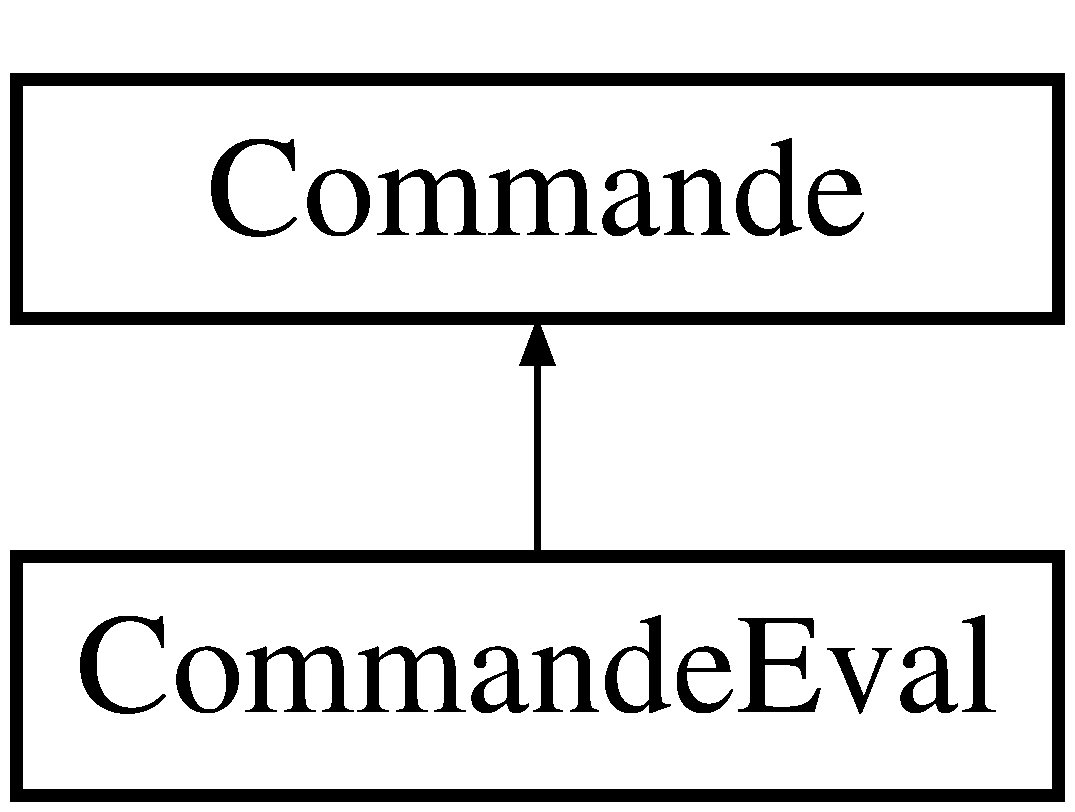
\includegraphics[height=2.000000cm]{class_commande_eval}
\end{center}
\end{figure}
\subsection*{Public Member Functions}
\begin{DoxyCompactItemize}
\item 
\hyperlink{class_commande_eval_ae7f29a48c48f9aaa6f218cb1642630eb}{Commande\-Eval} (\hyperlink{class_pile}{Pile} $\ast$p, \hyperlink{class_constante}{Constante} $\ast$c)
\begin{DoxyCompactList}\small\item\em constructeur. \end{DoxyCompactList}\item 
\hyperlink{class_commande_eval_ac545d7ad1c16bc7780132b1be79a137f}{$\sim$\-Commande\-Eval} ()
\begin{DoxyCompactList}\small\item\em destructeur. \end{DoxyCompactList}\item 
\hypertarget{class_commande_eval_ae16c7e11ada97aba12e9dfbaab0e8fa6}{void \hyperlink{class_commande_eval_ae16c7e11ada97aba12e9dfbaab0e8fa6}{Vider} ()}\label{class_commande_eval_ae16c7e11ada97aba12e9dfbaab0e8fa6}

\begin{DoxyCompactList}\small\item\em vide les piles de la commande. \end{DoxyCompactList}\item 
void \hyperlink{class_commande_eval_ad0055f5193a3d5fc0f7a3ee9fdcb09cb}{add\-Commande} (\hyperlink{class_commande}{Commande} $\ast$c)
\begin{DoxyCompactList}\small\item\em empile les pointeurs de commande dans p\-Commande \end{DoxyCompactList}\item 
void \hyperlink{class_commande_eval_a9a719eb128529581ef697284231bc805}{Do} ()
\begin{DoxyCompactList}\small\item\em executer l'operation \end{DoxyCompactList}\item 
void \hyperlink{class_commande_eval_a7bb0e495e43a30e5b7f0bf0d47cd37cf}{Undo} ()
\begin{DoxyCompactList}\small\item\em executer l'operation inverse \end{DoxyCompactList}\end{DoxyCompactItemize}


\subsection{Detailed Description}
\hyperlink{class_commande_eval}{Commande\-Eval} class. 

commande de la fonction eval. 

\subsection{Constructor \& Destructor Documentation}
\hypertarget{class_commande_eval_ae7f29a48c48f9aaa6f218cb1642630eb}{\index{Commande\-Eval@{Commande\-Eval}!Commande\-Eval@{Commande\-Eval}}
\index{Commande\-Eval@{Commande\-Eval}!CommandeEval@{Commande\-Eval}}
\subsubsection[{Commande\-Eval}]{\setlength{\rightskip}{0pt plus 5cm}Commande\-Eval\-::\-Commande\-Eval (
\begin{DoxyParamCaption}
\item[{{\bf Pile} $\ast$}]{p, }
\item[{{\bf Constante} $\ast$}]{c}
\end{DoxyParamCaption}
)\hspace{0.3cm}{\ttfamily [inline]}}}\label{class_commande_eval_ae7f29a48c48f9aaa6f218cb1642630eb}


constructeur. 


\begin{DoxyParams}{Parameters}
{\em c} & pointeur la constante expression evaluee \\
\hline
{\em p} & pointeur vers la pile stockant la commande \\
\hline
\end{DoxyParams}
\hypertarget{class_commande_eval_ac545d7ad1c16bc7780132b1be79a137f}{\index{Commande\-Eval@{Commande\-Eval}!$\sim$\-Commande\-Eval@{$\sim$\-Commande\-Eval}}
\index{$\sim$\-Commande\-Eval@{$\sim$\-Commande\-Eval}!CommandeEval@{Commande\-Eval}}
\subsubsection[{$\sim$\-Commande\-Eval}]{\setlength{\rightskip}{0pt plus 5cm}Commande\-Eval\-::$\sim$\-Commande\-Eval (
\begin{DoxyParamCaption}
{}
\end{DoxyParamCaption}
)\hspace{0.3cm}{\ttfamily [inline]}}}\label{class_commande_eval_ac545d7ad1c16bc7780132b1be79a137f}


destructeur. 

detruit la commande et les commandes de la pile p\-Commande 

\subsection{Member Function Documentation}
\hypertarget{class_commande_eval_ad0055f5193a3d5fc0f7a3ee9fdcb09cb}{\index{Commande\-Eval@{Commande\-Eval}!add\-Commande@{add\-Commande}}
\index{add\-Commande@{add\-Commande}!CommandeEval@{Commande\-Eval}}
\subsubsection[{add\-Commande}]{\setlength{\rightskip}{0pt plus 5cm}void Commande\-Eval\-::add\-Commande (
\begin{DoxyParamCaption}
\item[{{\bf Commande} $\ast$}]{c}
\end{DoxyParamCaption}
)\hspace{0.3cm}{\ttfamily [inline]}}}\label{class_commande_eval_ad0055f5193a3d5fc0f7a3ee9fdcb09cb}


empile les pointeurs de commande dans p\-Commande 


\begin{DoxyParams}{Parameters}
{\em c} & pointeur vers la commande a stocker \\
\hline
\end{DoxyParams}
\hypertarget{class_commande_eval_a9a719eb128529581ef697284231bc805}{\index{Commande\-Eval@{Commande\-Eval}!Do@{Do}}
\index{Do@{Do}!CommandeEval@{Commande\-Eval}}
\subsubsection[{Do}]{\setlength{\rightskip}{0pt plus 5cm}void Commande\-Eval\-::\-Do (
\begin{DoxyParamCaption}
{}
\end{DoxyParamCaption}
)\hspace{0.3cm}{\ttfamily [virtual]}}}\label{class_commande_eval_a9a719eb128529581ef697284231bc805}


executer l'operation 

execute l'ensemble des \hyperlink{class_commande_eval_a9a719eb128529581ef697284231bc805}{Do()} des commandes de la pile 

Implements \hyperlink{class_commande_a9fc0c740359ac4f0d34b9f109e3c0155}{Commande}.

\hypertarget{class_commande_eval_a7bb0e495e43a30e5b7f0bf0d47cd37cf}{\index{Commande\-Eval@{Commande\-Eval}!Undo@{Undo}}
\index{Undo@{Undo}!CommandeEval@{Commande\-Eval}}
\subsubsection[{Undo}]{\setlength{\rightskip}{0pt plus 5cm}void Commande\-Eval\-::\-Undo (
\begin{DoxyParamCaption}
{}
\end{DoxyParamCaption}
)\hspace{0.3cm}{\ttfamily [virtual]}}}\label{class_commande_eval_a7bb0e495e43a30e5b7f0bf0d47cd37cf}


executer l'operation inverse 

execute l'ensemble des \hyperlink{class_commande_eval_a7bb0e495e43a30e5b7f0bf0d47cd37cf}{Undo()} des commandes de la pile 

Implements \hyperlink{class_commande_a8523106c6ca6cc7c04323a641c16e563}{Commande}.



The documentation for this class was generated from the following files\-:\begin{DoxyCompactItemize}
\item 
E\-:/\-Dropbox/\-U\-T\-C/\-G\-I02/\-L\-O21/\-Calculatrice/commande.\-h\item 
E\-:/\-Dropbox/\-U\-T\-C/\-G\-I02/\-L\-O21/\-Calculatrice/commande.\-cpp\end{DoxyCompactItemize}

\hypertarget{class_commande_swap}{\section{Commande\-Swap Class Reference}
\label{class_commande_swap}\index{Commande\-Swap@{Commande\-Swap}}
}


\hyperlink{class_commande_swap}{Commande\-Swap} class.  




{\ttfamily \#include $<$commande.\-h$>$}

Inheritance diagram for Commande\-Swap\-:\begin{figure}[H]
\begin{center}
\leavevmode
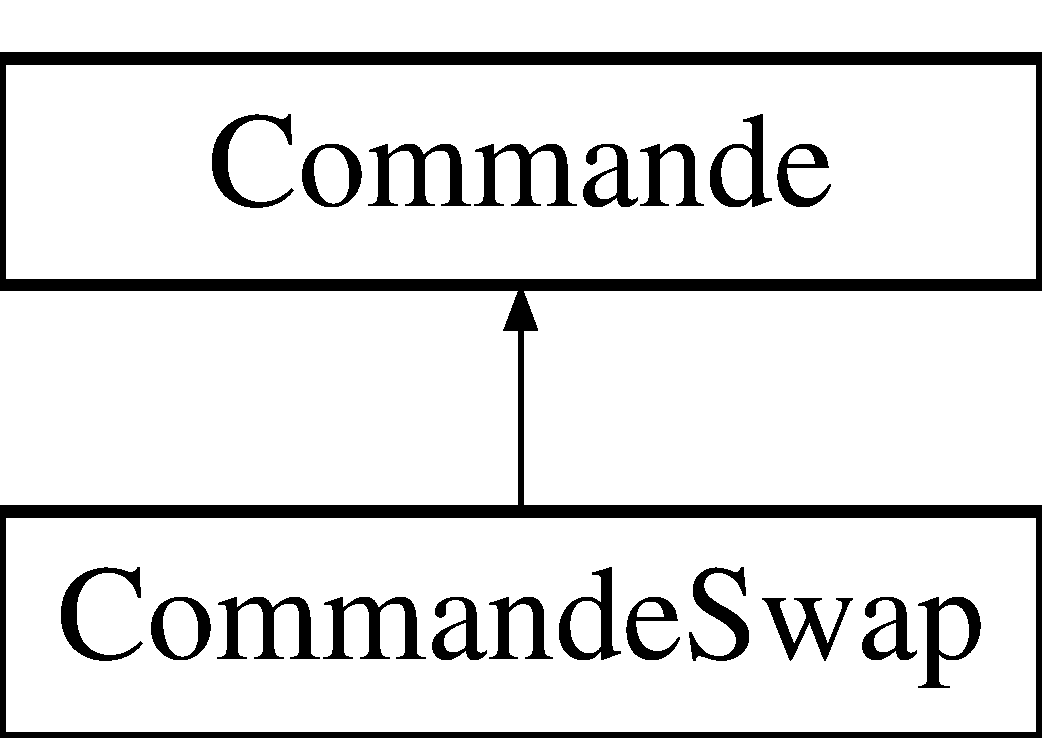
\includegraphics[height=2.000000cm]{class_commande_swap}
\end{center}
\end{figure}
\subsection*{Public Member Functions}
\begin{DoxyCompactItemize}
\item 
\hyperlink{class_commande_swap_a43a2f1b3aecdecc4fb14beb87783d9a2}{Commande\-Swap} (\hyperlink{class_pile}{Pile} $\ast$p)
\begin{DoxyCompactList}\small\item\em constructeur. \end{DoxyCompactList}\item 
\hypertarget{class_commande_swap_aaf63b2e5b1b4a6f5dbe6ae54641cac8b}{\hyperlink{class_commande_swap_aaf63b2e5b1b4a6f5dbe6ae54641cac8b}{$\sim$\-Commande\-Swap} ()}\label{class_commande_swap_aaf63b2e5b1b4a6f5dbe6ae54641cac8b}

\begin{DoxyCompactList}\small\item\em destructeur. \end{DoxyCompactList}\item 
\hypertarget{class_commande_swap_a5fcff8fc75c894dd46431280dddeba1e}{void \hyperlink{class_commande_swap_a5fcff8fc75c894dd46431280dddeba1e}{Vider} ()}\label{class_commande_swap_a5fcff8fc75c894dd46431280dddeba1e}

\begin{DoxyCompactList}\small\item\em vide le contenu de la pile old\-Const \end{DoxyCompactList}\item 
void \hyperlink{class_commande_swap_ac633e1a690413c200a11638d69f06afb}{add\-Old} (\hyperlink{class_constante}{Constante} $\ast$c)
\begin{DoxyCompactList}\small\item\em ajoute la constante sur la pile old\-Const \end{DoxyCompactList}\item 
\hypertarget{class_commande_swap_a955666912c56a1c71b7579d837bc3762}{void \hyperlink{class_commande_swap_a955666912c56a1c71b7579d837bc3762}{Do} ()}\label{class_commande_swap_a955666912c56a1c71b7579d837bc3762}

\begin{DoxyCompactList}\small\item\em effectue un swap sur la pile \end{DoxyCompactList}\item 
\hypertarget{class_commande_swap_a9d2f74b321b071df3a81abf2f1f0b40d}{void \hyperlink{class_commande_swap_a9d2f74b321b071df3a81abf2f1f0b40d}{Undo} ()}\label{class_commande_swap_a9d2f74b321b071df3a81abf2f1f0b40d}

\begin{DoxyCompactList}\small\item\em ajoute les parametres de la pile old\-Const puis effectue un swap sur la pile puis ajoute de nouveau les parametres de old\-Const \end{DoxyCompactList}\end{DoxyCompactItemize}


\subsection{Detailed Description}
\hyperlink{class_commande_swap}{Commande\-Swap} class. 

commande de la fonction swap. 

\subsection{Constructor \& Destructor Documentation}
\hypertarget{class_commande_swap_a43a2f1b3aecdecc4fb14beb87783d9a2}{\index{Commande\-Swap@{Commande\-Swap}!Commande\-Swap@{Commande\-Swap}}
\index{Commande\-Swap@{Commande\-Swap}!CommandeSwap@{Commande\-Swap}}
\subsubsection[{Commande\-Swap}]{\setlength{\rightskip}{0pt plus 5cm}Commande\-Swap\-::\-Commande\-Swap (
\begin{DoxyParamCaption}
\item[{{\bf Pile} $\ast$}]{p}
\end{DoxyParamCaption}
)\hspace{0.3cm}{\ttfamily [inline]}}}\label{class_commande_swap_a43a2f1b3aecdecc4fb14beb87783d9a2}


constructeur. 


\begin{DoxyParams}{Parameters}
{\em p} & Pointeur vers la pile stockant la commande \\
\hline
\end{DoxyParams}


\subsection{Member Function Documentation}
\hypertarget{class_commande_swap_ac633e1a690413c200a11638d69f06afb}{\index{Commande\-Swap@{Commande\-Swap}!add\-Old@{add\-Old}}
\index{add\-Old@{add\-Old}!CommandeSwap@{Commande\-Swap}}
\subsubsection[{add\-Old}]{\setlength{\rightskip}{0pt plus 5cm}void Commande\-Swap\-::add\-Old (
\begin{DoxyParamCaption}
\item[{{\bf Constante} $\ast$}]{c}
\end{DoxyParamCaption}
)}}\label{class_commande_swap_ac633e1a690413c200a11638d69f06afb}


ajoute la constante sur la pile old\-Const 


\begin{DoxyParams}{Parameters}
{\em c} & Pointeur vers la \hyperlink{class_constante}{Constante} a stocker \\
\hline
\end{DoxyParams}


The documentation for this class was generated from the following files\-:\begin{DoxyCompactItemize}
\item 
E\-:/\-Dropbox/\-U\-T\-C/\-G\-I02/\-L\-O21/\-Calculatrice/commande.\-h\item 
E\-:/\-Dropbox/\-U\-T\-C/\-G\-I02/\-L\-O21/\-Calculatrice/commande.\-cpp\end{DoxyCompactItemize}

\hypertarget{class_constante}{\section{Constante Class Reference}
\label{class_constante}\index{Constante@{Constante}}
}


\hyperlink{class_constante}{Constante} class.  




{\ttfamily \#include $<$constante.\-h$>$}

Inheritance diagram for Constante\-:\begin{figure}[H]
\begin{center}
\leavevmode
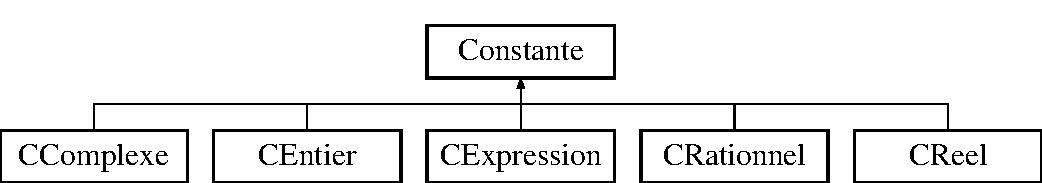
\includegraphics[height=2.000000cm]{class_constante}
\end{center}
\end{figure}
\subsection*{Public Member Functions}
\begin{DoxyCompactItemize}
\item 
virtual Q\-String \hyperlink{class_constante_a93d89080856c972bdebc3619fc957f52}{get\-Valueto\-String} () const =0
\begin{DoxyCompactList}\small\item\em retourne le contenu de la constante sous forme de texte \end{DoxyCompactList}\item 
virtual \hyperlink{class_constante}{Constante} $\ast$ \hyperlink{class_constante_ae1c9e9fa9b3272e37bdb292509741831}{operator+} (\hyperlink{class_constante}{Constante} \&c1)=0
\begin{DoxyCompactList}\small\item\em retourne le resultat de l'operation + entre deux constantes \end{DoxyCompactList}\item 
virtual \hyperlink{class_constante}{Constante} $\ast$ \hyperlink{class_constante_a9d0df3d484c2d87556cb4faa73606862}{operator-\/} (\hyperlink{class_constante}{Constante} \&c1)=0
\begin{DoxyCompactList}\small\item\em retourne le resultat de l'operation -\/ entre deux constantes \end{DoxyCompactList}\item 
virtual \hyperlink{class_constante}{Constante} $\ast$ \hyperlink{class_constante_ae7c4cf6a493277ec98ae346e13bbf82a}{operator$\ast$} (\hyperlink{class_constante}{Constante} \&c1)=0
\begin{DoxyCompactList}\small\item\em retourne le resultat de l'operation $\ast$ entre deux constantes \end{DoxyCompactList}\item 
virtual \hyperlink{class_constante}{Constante} $\ast$ \hyperlink{class_constante_af83c6680a11bc9ca5db49a32864151dd}{operator/} (\hyperlink{class_constante}{Constante} \&c1)=0
\begin{DoxyCompactList}\small\item\em retourne le resultat de l'operation / entre deux constantes \end{DoxyCompactList}\item 
virtual \hyperlink{class_constante}{Constante} $\ast$ \hyperlink{class_constante_addd94a5006b4ed68cc0d1d7b5864e10a}{get\-Copy} ()=0
\begin{DoxyCompactList}\small\item\em retourne une copie de la constante \end{DoxyCompactList}\end{DoxyCompactItemize}


\subsection{Detailed Description}
\hyperlink{class_constante}{Constante} class. 

classe virtuelle des Constantes 

\subsection{Member Function Documentation}
\hypertarget{class_constante_addd94a5006b4ed68cc0d1d7b5864e10a}{\index{Constante@{Constante}!get\-Copy@{get\-Copy}}
\index{get\-Copy@{get\-Copy}!Constante@{Constante}}
\subsubsection[{get\-Copy}]{\setlength{\rightskip}{0pt plus 5cm}virtual {\bf Constante}$\ast$ Constante\-::get\-Copy (
\begin{DoxyParamCaption}
{}
\end{DoxyParamCaption}
)\hspace{0.3cm}{\ttfamily [pure virtual]}}}\label{class_constante_addd94a5006b4ed68cc0d1d7b5864e10a}


retourne une copie de la constante 

\begin{DoxyReturn}{Returns}
pointeur vers une copie de la constante 
\end{DoxyReturn}


Implemented in \hyperlink{class_c_complexe_a5afb89b25938e8c6b457de3b80da5cb0}{C\-Complexe}, \hyperlink{class_c_expression_a0fbadaea165e135c3e12bc35b31a2d55}{C\-Expression}, \hyperlink{class_c_rationnel_aba8783eae5fcf033e80ebf03c4776964}{C\-Rationnel}, \hyperlink{class_c_reel_a7971d82193e3305f266f69547cad8bb7}{C\-Reel}, and \hyperlink{class_c_entier_a48a8a57548157ff88606891b585aa04a}{C\-Entier}.

\hypertarget{class_constante_a93d89080856c972bdebc3619fc957f52}{\index{Constante@{Constante}!get\-Valueto\-String@{get\-Valueto\-String}}
\index{get\-Valueto\-String@{get\-Valueto\-String}!Constante@{Constante}}
\subsubsection[{get\-Valueto\-String}]{\setlength{\rightskip}{0pt plus 5cm}virtual Q\-String Constante\-::get\-Valueto\-String (
\begin{DoxyParamCaption}
{}
\end{DoxyParamCaption}
) const\hspace{0.3cm}{\ttfamily [pure virtual]}}}\label{class_constante_a93d89080856c972bdebc3619fc957f52}


retourne le contenu de la constante sous forme de texte 

\begin{DoxyReturn}{Returns}
Q\-String valeur formatee de la constante 
\end{DoxyReturn}


Implemented in \hyperlink{class_c_complexe_a2ac287ee5fac2c2365fe618f47d235dc}{C\-Complexe}, \hyperlink{class_c_expression_a642f89de974553f82cff731f6d83fea6}{C\-Expression}, \hyperlink{class_c_rationnel_ab35caed898661511138268547b27514a}{C\-Rationnel}, \hyperlink{class_c_reel_a4f8123c4f5659383d05ead9d02b221ec}{C\-Reel}, and \hyperlink{class_c_entier_ae25f1f0b9422e1d7f256d8e15249e5b6}{C\-Entier}.

\hypertarget{class_constante_ae7c4cf6a493277ec98ae346e13bbf82a}{\index{Constante@{Constante}!operator$\ast$@{operator$\ast$}}
\index{operator$\ast$@{operator$\ast$}!Constante@{Constante}}
\subsubsection[{operator$\ast$}]{\setlength{\rightskip}{0pt plus 5cm}virtual {\bf Constante}$\ast$ Constante\-::operator$\ast$ (
\begin{DoxyParamCaption}
\item[{{\bf Constante} \&}]{c1}
\end{DoxyParamCaption}
)\hspace{0.3cm}{\ttfamily [pure virtual]}}}\label{class_constante_ae7c4cf6a493277ec98ae346e13bbf82a}


retourne le resultat de l'operation $\ast$ entre deux constantes 


\begin{DoxyParams}{Parameters}
{\em c1} & reference vers le deuxieme operande de type \hyperlink{class_constante}{Constante} \\
\hline
\end{DoxyParams}
\begin{DoxyReturn}{Returns}
un pointeur \hyperlink{class_constante}{Constante} sur le resultat 
\end{DoxyReturn}


Implemented in \hyperlink{class_c_complexe_aa0d80726cdd5b1aba17ac25c2bed1194}{C\-Complexe}, \hyperlink{class_c_expression_a0bcd0e43fe294b187d7ff7240a246ac2}{C\-Expression}, \hyperlink{class_c_rationnel_a1e06a24de386d66b8e15d53383e43694}{C\-Rationnel}, \hyperlink{class_c_reel_ac0730d78556c60bf9824fff423554033}{C\-Reel}, and \hyperlink{class_c_entier_a2ca548de9fa6c4446d4bd16c0061d3d9}{C\-Entier}.

\hypertarget{class_constante_ae1c9e9fa9b3272e37bdb292509741831}{\index{Constante@{Constante}!operator+@{operator+}}
\index{operator+@{operator+}!Constante@{Constante}}
\subsubsection[{operator+}]{\setlength{\rightskip}{0pt plus 5cm}virtual {\bf Constante}$\ast$ Constante\-::operator+ (
\begin{DoxyParamCaption}
\item[{{\bf Constante} \&}]{c1}
\end{DoxyParamCaption}
)\hspace{0.3cm}{\ttfamily [pure virtual]}}}\label{class_constante_ae1c9e9fa9b3272e37bdb292509741831}


retourne le resultat de l'operation + entre deux constantes 


\begin{DoxyParams}{Parameters}
{\em c1} & reference vers le deuxieme operande de type \hyperlink{class_constante}{Constante} \\
\hline
\end{DoxyParams}
\begin{DoxyReturn}{Returns}
un pointeur \hyperlink{class_constante}{Constante} sur le resultat 
\end{DoxyReturn}


Implemented in \hyperlink{class_c_complexe_a3ff3a06dde38c3fba33fafbef7b3cd99}{C\-Complexe}, \hyperlink{class_c_expression_a673be1d66195b8ee7fac79b53d8cf371}{C\-Expression}, \hyperlink{class_c_rationnel_ace7aee26a004983cebb7336de1079855}{C\-Rationnel}, \hyperlink{class_c_reel_a61a8eb92280d208f9fffa699f9be989f}{C\-Reel}, and \hyperlink{class_c_entier_a90d87411cff696ada012b426082f9c87}{C\-Entier}.

\hypertarget{class_constante_a9d0df3d484c2d87556cb4faa73606862}{\index{Constante@{Constante}!operator-\/@{operator-\/}}
\index{operator-\/@{operator-\/}!Constante@{Constante}}
\subsubsection[{operator-\/}]{\setlength{\rightskip}{0pt plus 5cm}virtual {\bf Constante}$\ast$ Constante\-::operator-\/ (
\begin{DoxyParamCaption}
\item[{{\bf Constante} \&}]{c1}
\end{DoxyParamCaption}
)\hspace{0.3cm}{\ttfamily [pure virtual]}}}\label{class_constante_a9d0df3d484c2d87556cb4faa73606862}


retourne le resultat de l'operation -\/ entre deux constantes 


\begin{DoxyParams}{Parameters}
{\em c1} & reference vers le deuxieme operande de type \hyperlink{class_constante}{Constante} \\
\hline
\end{DoxyParams}
\begin{DoxyReturn}{Returns}
un pointeur \hyperlink{class_constante}{Constante} sur le resultat 
\end{DoxyReturn}


Implemented in \hyperlink{class_c_complexe_a2661c1f2dedc3f417af1a941f11ca583}{C\-Complexe}, \hyperlink{class_c_expression_af7fdc3e9fa28257c0cdfed04995cbe8e}{C\-Expression}, \hyperlink{class_c_rationnel_a79afb1dec74f4aed07722a1d496837c4}{C\-Rationnel}, \hyperlink{class_c_reel_abb39aa0b30a2673bdc34b808da836006}{C\-Reel}, and \hyperlink{class_c_entier_a5f07b4783dfcfb024cf8c72caac64be7}{C\-Entier}.

\hypertarget{class_constante_af83c6680a11bc9ca5db49a32864151dd}{\index{Constante@{Constante}!operator/@{operator/}}
\index{operator/@{operator/}!Constante@{Constante}}
\subsubsection[{operator/}]{\setlength{\rightskip}{0pt plus 5cm}virtual {\bf Constante}$\ast$ Constante\-::operator/ (
\begin{DoxyParamCaption}
\item[{{\bf Constante} \&}]{c1}
\end{DoxyParamCaption}
)\hspace{0.3cm}{\ttfamily [pure virtual]}}}\label{class_constante_af83c6680a11bc9ca5db49a32864151dd}


retourne le resultat de l'operation / entre deux constantes 


\begin{DoxyParams}{Parameters}
{\em c1} & reference vers le deuxieme operande de type \hyperlink{class_constante}{Constante} \\
\hline
\end{DoxyParams}
\begin{DoxyReturn}{Returns}
un pointeur \hyperlink{class_constante}{Constante} sur le resultat 
\end{DoxyReturn}


Implemented in \hyperlink{class_c_complexe_a518ad5669537f64418ef6007687a3297}{C\-Complexe}, \hyperlink{class_c_expression_a92584ee17ad2f42488a37aa991fa3352}{C\-Expression}, \hyperlink{class_c_rationnel_abe7c61d484fe7d3062f45ff43a18cf23}{C\-Rationnel}, \hyperlink{class_c_reel_a12bf069085a82f9d6b99482f538258f9}{C\-Reel}, and \hyperlink{class_c_entier_a0cfb4e65d73cbe8e55be9ade1948d8ec}{C\-Entier}.



The documentation for this class was generated from the following file\-:\begin{DoxyCompactItemize}
\item 
E\-:/\-Dropbox/\-U\-T\-C/\-G\-I02/\-L\-O21/\-Calculatrice/constante.\-h\end{DoxyCompactItemize}

\hypertarget{class_c_rationnel}{\section{C\-Rationnel Class Reference}
\label{class_c_rationnel}\index{C\-Rationnel@{C\-Rationnel}}
}


\hyperlink{class_c_rationnel}{C\-Rationnel} class.  




{\ttfamily \#include $<$constante.\-h$>$}

Inheritance diagram for C\-Rationnel\-:\begin{figure}[H]
\begin{center}
\leavevmode
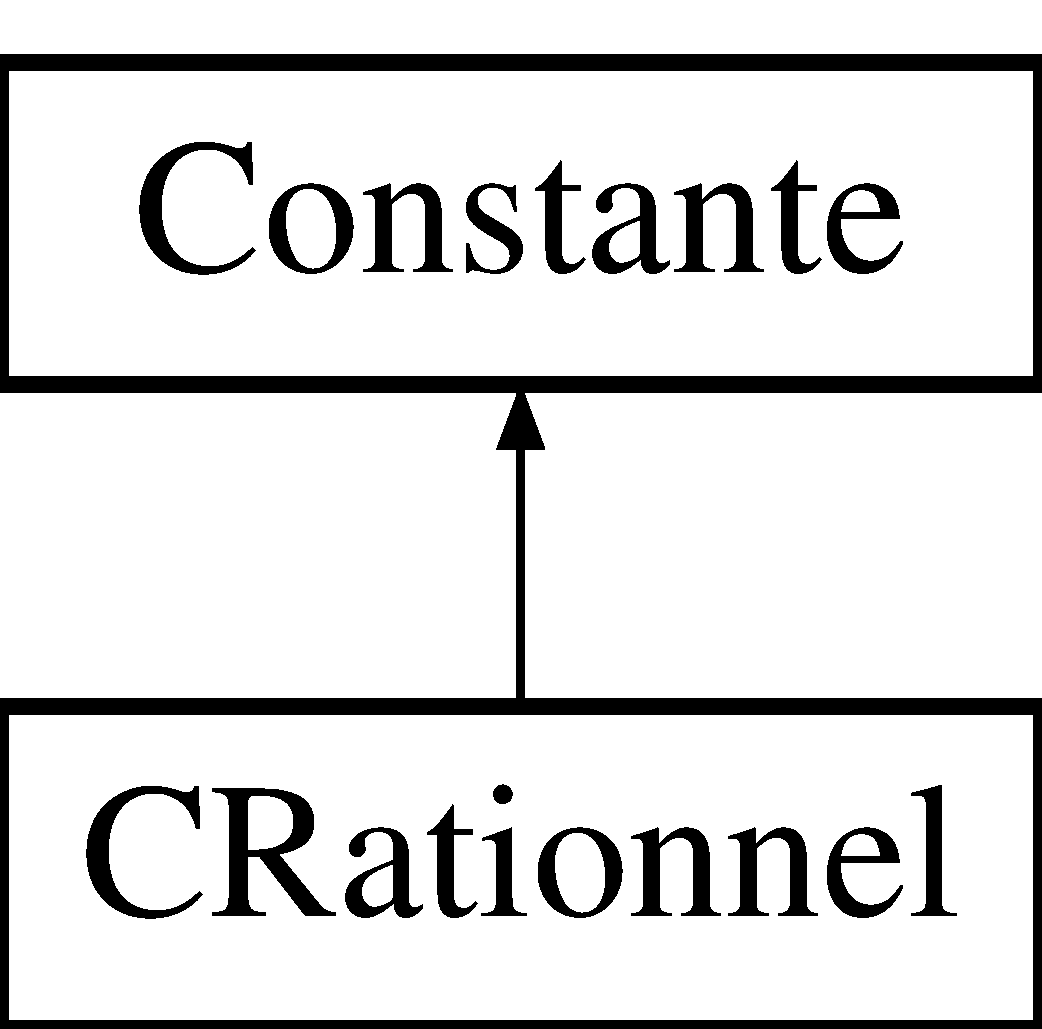
\includegraphics[height=2.000000cm]{class_c_rationnel}
\end{center}
\end{figure}
\subsection*{Public Member Functions}
\begin{DoxyCompactItemize}
\item 
\hyperlink{class_c_rationnel_abb873462d03ad1522ff11f6a673eec43}{C\-Rationnel} (int n, int d)
\begin{DoxyCompactList}\small\item\em constructeur. \end{DoxyCompactList}\item 
\hyperlink{class_c_rationnel_a73f3e9dc846975b3364596a656bd9a11}{C\-Rationnel} (const \hyperlink{class_c_rationnel}{C\-Rationnel} \&c)
\begin{DoxyCompactList}\small\item\em constructeur par copie. \end{DoxyCompactList}\item 
\hyperlink{class_c_rationnel_ac046cfa1329cc37a236fe3d3adbd9663}{C\-Rationnel} (float f)
\begin{DoxyCompactList}\small\item\em constructeur avec float. \end{DoxyCompactList}\item 
\hyperlink{class_constante}{Constante} $\ast$ \hyperlink{class_c_rationnel_aba8783eae5fcf033e80ebf03c4776964}{get\-Copy} ()
\begin{DoxyCompactList}\small\item\em retourne une copie de la constante \end{DoxyCompactList}\item 
int \hyperlink{class_c_rationnel_a1d67342e386a8e3ad70ed3413f793c4f}{get\-Num} () const 
\begin{DoxyCompactList}\small\item\em renvoit le numerateur. \end{DoxyCompactList}\item 
int \hyperlink{class_c_rationnel_acad7d65e21a390f4fb253767413a1131}{get\-Denom} () const 
\begin{DoxyCompactList}\small\item\em renvoit le denominateur. \end{DoxyCompactList}\item 
void \hyperlink{class_c_rationnel_a361e29398792bc3d00d65c99d1dd2350}{set\-Num} (int e)
\begin{DoxyCompactList}\small\item\em affect un numerateur. \end{DoxyCompactList}\item 
void \hyperlink{class_c_rationnel_a3e49f03bc4501f6d71c7c82897dc21c6}{set\-Denom} (int e)
\begin{DoxyCompactList}\small\item\em affect un denominateur. \end{DoxyCompactList}\item 
Q\-String \hyperlink{class_c_rationnel_ab35caed898661511138268547b27514a}{get\-Valueto\-String} () const 
\begin{DoxyCompactList}\small\item\em retourne le contenu de la constante sous forme de texte \end{DoxyCompactList}\item 
\hyperlink{class_constante}{Constante} $\ast$ \hyperlink{class_c_rationnel_ace7aee26a004983cebb7336de1079855}{operator+} (\hyperlink{class_constante}{Constante} \&c1)
\begin{DoxyCompactList}\small\item\em retourne le resultat de l'operation + entre deux constantes \end{DoxyCompactList}\item 
\hyperlink{class_constante}{Constante} $\ast$ \hyperlink{class_c_rationnel_a79afb1dec74f4aed07722a1d496837c4}{operator-\/} (\hyperlink{class_constante}{Constante} \&c1)
\begin{DoxyCompactList}\small\item\em retourne le resultat de l'operation -\/ entre deux constantes \end{DoxyCompactList}\item 
\hyperlink{class_constante}{Constante} $\ast$ \hyperlink{class_c_rationnel_a1e06a24de386d66b8e15d53383e43694}{operator$\ast$} (\hyperlink{class_constante}{Constante} \&c1)
\begin{DoxyCompactList}\small\item\em retourne le resultat de l'operation $\ast$ entre deux constantes \end{DoxyCompactList}\item 
\hyperlink{class_constante}{Constante} $\ast$ \hyperlink{class_c_rationnel_abe7c61d484fe7d3062f45ff43a18cf23}{operator/} (\hyperlink{class_constante}{Constante} \&c1)
\begin{DoxyCompactList}\small\item\em retourne le resultat de l'operation / entre deux constantes \end{DoxyCompactList}\item 
\hypertarget{class_c_rationnel_a49a7282a978004d90500c327f0595af4}{\hyperlink{class_c_rationnel_a49a7282a978004d90500c327f0595af4}{$\sim$\-C\-Rationnel} ()}\label{class_c_rationnel_a49a7282a978004d90500c327f0595af4}

\begin{DoxyCompactList}\small\item\em destructeur. \end{DoxyCompactList}\end{DoxyCompactItemize}


\subsection{Detailed Description}
\hyperlink{class_c_rationnel}{C\-Rationnel} class. 

classe des types rationnels 

\subsection{Constructor \& Destructor Documentation}
\hypertarget{class_c_rationnel_abb873462d03ad1522ff11f6a673eec43}{\index{C\-Rationnel@{C\-Rationnel}!C\-Rationnel@{C\-Rationnel}}
\index{C\-Rationnel@{C\-Rationnel}!CRationnel@{C\-Rationnel}}
\subsubsection[{C\-Rationnel}]{\setlength{\rightskip}{0pt plus 5cm}C\-Rationnel\-::\-C\-Rationnel (
\begin{DoxyParamCaption}
\item[{int}]{n, }
\item[{int}]{d}
\end{DoxyParamCaption}
)\hspace{0.3cm}{\ttfamily [inline]}}}\label{class_c_rationnel_abb873462d03ad1522ff11f6a673eec43}


constructeur. 


\begin{DoxyParams}{Parameters}
{\em n} & numerateur \\
\hline
{\em d} & denominateur \\
\hline
\end{DoxyParams}
\hypertarget{class_c_rationnel_a73f3e9dc846975b3364596a656bd9a11}{\index{C\-Rationnel@{C\-Rationnel}!C\-Rationnel@{C\-Rationnel}}
\index{C\-Rationnel@{C\-Rationnel}!CRationnel@{C\-Rationnel}}
\subsubsection[{C\-Rationnel}]{\setlength{\rightskip}{0pt plus 5cm}C\-Rationnel\-::\-C\-Rationnel (
\begin{DoxyParamCaption}
\item[{const {\bf C\-Rationnel} \&}]{c}
\end{DoxyParamCaption}
)\hspace{0.3cm}{\ttfamily [inline]}}}\label{class_c_rationnel_a73f3e9dc846975b3364596a656bd9a11}


constructeur par copie. 


\begin{DoxyParams}{Parameters}
{\em c} & reference vers le \hyperlink{class_c_rationnel}{C\-Rationnel} a copier \\
\hline
\end{DoxyParams}
\hypertarget{class_c_rationnel_ac046cfa1329cc37a236fe3d3adbd9663}{\index{C\-Rationnel@{C\-Rationnel}!C\-Rationnel@{C\-Rationnel}}
\index{C\-Rationnel@{C\-Rationnel}!CRationnel@{C\-Rationnel}}
\subsubsection[{C\-Rationnel}]{\setlength{\rightskip}{0pt plus 5cm}C\-Rationnel\-::\-C\-Rationnel (
\begin{DoxyParamCaption}
\item[{float}]{f}
\end{DoxyParamCaption}
)\hspace{0.3cm}{\ttfamily [inline]}}}\label{class_c_rationnel_ac046cfa1329cc37a236fe3d3adbd9663}


constructeur avec float. 


\begin{DoxyParams}{Parameters}
{\em f} & float a convertir \\
\hline
\end{DoxyParams}


\subsection{Member Function Documentation}
\hypertarget{class_c_rationnel_aba8783eae5fcf033e80ebf03c4776964}{\index{C\-Rationnel@{C\-Rationnel}!get\-Copy@{get\-Copy}}
\index{get\-Copy@{get\-Copy}!CRationnel@{C\-Rationnel}}
\subsubsection[{get\-Copy}]{\setlength{\rightskip}{0pt plus 5cm}{\bf Constante}$\ast$ C\-Rationnel\-::get\-Copy (
\begin{DoxyParamCaption}
{}
\end{DoxyParamCaption}
)\hspace{0.3cm}{\ttfamily [inline]}, {\ttfamily [virtual]}}}\label{class_c_rationnel_aba8783eae5fcf033e80ebf03c4776964}


retourne une copie de la constante 

\begin{DoxyReturn}{Returns}
pointeur vers une copie de la constante 
\end{DoxyReturn}


Implements \hyperlink{class_constante_addd94a5006b4ed68cc0d1d7b5864e10a}{Constante}.

\hypertarget{class_c_rationnel_acad7d65e21a390f4fb253767413a1131}{\index{C\-Rationnel@{C\-Rationnel}!get\-Denom@{get\-Denom}}
\index{get\-Denom@{get\-Denom}!CRationnel@{C\-Rationnel}}
\subsubsection[{get\-Denom}]{\setlength{\rightskip}{0pt plus 5cm}int C\-Rationnel\-::get\-Denom (
\begin{DoxyParamCaption}
{}
\end{DoxyParamCaption}
) const\hspace{0.3cm}{\ttfamily [inline]}}}\label{class_c_rationnel_acad7d65e21a390f4fb253767413a1131}


renvoit le denominateur. 

\begin{DoxyReturn}{Returns}
denominateur integer 
\end{DoxyReturn}
\hypertarget{class_c_rationnel_a1d67342e386a8e3ad70ed3413f793c4f}{\index{C\-Rationnel@{C\-Rationnel}!get\-Num@{get\-Num}}
\index{get\-Num@{get\-Num}!CRationnel@{C\-Rationnel}}
\subsubsection[{get\-Num}]{\setlength{\rightskip}{0pt plus 5cm}int C\-Rationnel\-::get\-Num (
\begin{DoxyParamCaption}
{}
\end{DoxyParamCaption}
) const\hspace{0.3cm}{\ttfamily [inline]}}}\label{class_c_rationnel_a1d67342e386a8e3ad70ed3413f793c4f}


renvoit le numerateur. 

\begin{DoxyReturn}{Returns}
numerateur integer 
\end{DoxyReturn}
\hypertarget{class_c_rationnel_ab35caed898661511138268547b27514a}{\index{C\-Rationnel@{C\-Rationnel}!get\-Valueto\-String@{get\-Valueto\-String}}
\index{get\-Valueto\-String@{get\-Valueto\-String}!CRationnel@{C\-Rationnel}}
\subsubsection[{get\-Valueto\-String}]{\setlength{\rightskip}{0pt plus 5cm}Q\-String C\-Rationnel\-::get\-Valueto\-String (
\begin{DoxyParamCaption}
{}
\end{DoxyParamCaption}
) const\hspace{0.3cm}{\ttfamily [inline]}, {\ttfamily [virtual]}}}\label{class_c_rationnel_ab35caed898661511138268547b27514a}


retourne le contenu de la constante sous forme de texte 

\begin{DoxyReturn}{Returns}
Q\-String valeur formatee de la constante 
\end{DoxyReturn}


Implements \hyperlink{class_constante_a93d89080856c972bdebc3619fc957f52}{Constante}.

\hypertarget{class_c_rationnel_a1e06a24de386d66b8e15d53383e43694}{\index{C\-Rationnel@{C\-Rationnel}!operator$\ast$@{operator$\ast$}}
\index{operator$\ast$@{operator$\ast$}!CRationnel@{C\-Rationnel}}
\subsubsection[{operator$\ast$}]{\setlength{\rightskip}{0pt plus 5cm}{\bf Constante} $\ast$ C\-Rationnel\-::operator$\ast$ (
\begin{DoxyParamCaption}
\item[{{\bf Constante} \&}]{c1}
\end{DoxyParamCaption}
)\hspace{0.3cm}{\ttfamily [virtual]}}}\label{class_c_rationnel_a1e06a24de386d66b8e15d53383e43694}


retourne le resultat de l'operation $\ast$ entre deux constantes 


\begin{DoxyParams}{Parameters}
{\em c1} & reference vers le deuxieme operande de type \hyperlink{class_constante}{Constante} \\
\hline
\end{DoxyParams}
\begin{DoxyReturn}{Returns}
un pointeur \hyperlink{class_constante}{Constante} sur le resultat 
\end{DoxyReturn}


Implements \hyperlink{class_constante_ae7c4cf6a493277ec98ae346e13bbf82a}{Constante}.

\hypertarget{class_c_rationnel_ace7aee26a004983cebb7336de1079855}{\index{C\-Rationnel@{C\-Rationnel}!operator+@{operator+}}
\index{operator+@{operator+}!CRationnel@{C\-Rationnel}}
\subsubsection[{operator+}]{\setlength{\rightskip}{0pt plus 5cm}{\bf Constante} $\ast$ C\-Rationnel\-::operator+ (
\begin{DoxyParamCaption}
\item[{{\bf Constante} \&}]{c1}
\end{DoxyParamCaption}
)\hspace{0.3cm}{\ttfamily [virtual]}}}\label{class_c_rationnel_ace7aee26a004983cebb7336de1079855}


retourne le resultat de l'operation + entre deux constantes 


\begin{DoxyParams}{Parameters}
{\em c1} & reference vers le deuxieme operande de type \hyperlink{class_constante}{Constante} \\
\hline
\end{DoxyParams}
\begin{DoxyReturn}{Returns}
un pointeur \hyperlink{class_constante}{Constante} sur le resultat 
\end{DoxyReturn}


Implements \hyperlink{class_constante_ae1c9e9fa9b3272e37bdb292509741831}{Constante}.

\hypertarget{class_c_rationnel_a79afb1dec74f4aed07722a1d496837c4}{\index{C\-Rationnel@{C\-Rationnel}!operator-\/@{operator-\/}}
\index{operator-\/@{operator-\/}!CRationnel@{C\-Rationnel}}
\subsubsection[{operator-\/}]{\setlength{\rightskip}{0pt plus 5cm}{\bf Constante} $\ast$ C\-Rationnel\-::operator-\/ (
\begin{DoxyParamCaption}
\item[{{\bf Constante} \&}]{c1}
\end{DoxyParamCaption}
)\hspace{0.3cm}{\ttfamily [virtual]}}}\label{class_c_rationnel_a79afb1dec74f4aed07722a1d496837c4}


retourne le resultat de l'operation -\/ entre deux constantes 


\begin{DoxyParams}{Parameters}
{\em c1} & reference vers le deuxieme operande de type \hyperlink{class_constante}{Constante} \\
\hline
\end{DoxyParams}
\begin{DoxyReturn}{Returns}
un pointeur \hyperlink{class_constante}{Constante} sur le resultat 
\end{DoxyReturn}


Implements \hyperlink{class_constante_a9d0df3d484c2d87556cb4faa73606862}{Constante}.

\hypertarget{class_c_rationnel_abe7c61d484fe7d3062f45ff43a18cf23}{\index{C\-Rationnel@{C\-Rationnel}!operator/@{operator/}}
\index{operator/@{operator/}!CRationnel@{C\-Rationnel}}
\subsubsection[{operator/}]{\setlength{\rightskip}{0pt plus 5cm}{\bf Constante} $\ast$ C\-Rationnel\-::operator/ (
\begin{DoxyParamCaption}
\item[{{\bf Constante} \&}]{c1}
\end{DoxyParamCaption}
)\hspace{0.3cm}{\ttfamily [virtual]}}}\label{class_c_rationnel_abe7c61d484fe7d3062f45ff43a18cf23}


retourne le resultat de l'operation / entre deux constantes 


\begin{DoxyParams}{Parameters}
{\em c1} & reference vers le deuxieme operande de type \hyperlink{class_constante}{Constante} \\
\hline
\end{DoxyParams}
\begin{DoxyReturn}{Returns}
un pointeur \hyperlink{class_constante}{Constante} sur le resultat 
\end{DoxyReturn}


Implements \hyperlink{class_constante_af83c6680a11bc9ca5db49a32864151dd}{Constante}.

\hypertarget{class_c_rationnel_a3e49f03bc4501f6d71c7c82897dc21c6}{\index{C\-Rationnel@{C\-Rationnel}!set\-Denom@{set\-Denom}}
\index{set\-Denom@{set\-Denom}!CRationnel@{C\-Rationnel}}
\subsubsection[{set\-Denom}]{\setlength{\rightskip}{0pt plus 5cm}void C\-Rationnel\-::set\-Denom (
\begin{DoxyParamCaption}
\item[{int}]{e}
\end{DoxyParamCaption}
)\hspace{0.3cm}{\ttfamily [inline]}}}\label{class_c_rationnel_a3e49f03bc4501f6d71c7c82897dc21c6}


affect un denominateur. 


\begin{DoxyParams}{Parameters}
{\em e} & denominateur integer \\
\hline
\end{DoxyParams}
\hypertarget{class_c_rationnel_a361e29398792bc3d00d65c99d1dd2350}{\index{C\-Rationnel@{C\-Rationnel}!set\-Num@{set\-Num}}
\index{set\-Num@{set\-Num}!CRationnel@{C\-Rationnel}}
\subsubsection[{set\-Num}]{\setlength{\rightskip}{0pt plus 5cm}void C\-Rationnel\-::set\-Num (
\begin{DoxyParamCaption}
\item[{int}]{e}
\end{DoxyParamCaption}
)\hspace{0.3cm}{\ttfamily [inline]}}}\label{class_c_rationnel_a361e29398792bc3d00d65c99d1dd2350}


affect un numerateur. 


\begin{DoxyParams}{Parameters}
{\em e} & numerateur integer \\
\hline
\end{DoxyParams}


The documentation for this class was generated from the following files\-:\begin{DoxyCompactItemize}
\item 
E\-:/\-Dropbox/\-U\-T\-C/\-G\-I02/\-L\-O21/\-Calculatrice/constante.\-h\item 
E\-:/\-Dropbox/\-U\-T\-C/\-G\-I02/\-L\-O21/\-Calculatrice/constante.\-cpp\end{DoxyCompactItemize}

\hypertarget{class_c_reel}{\section{C\-Reel Class Reference}
\label{class_c_reel}\index{C\-Reel@{C\-Reel}}
}


\hyperlink{class_c_reel}{C\-Reel} class.  




{\ttfamily \#include $<$constante.\-h$>$}

Inheritance diagram for C\-Reel\-:\begin{figure}[H]
\begin{center}
\leavevmode
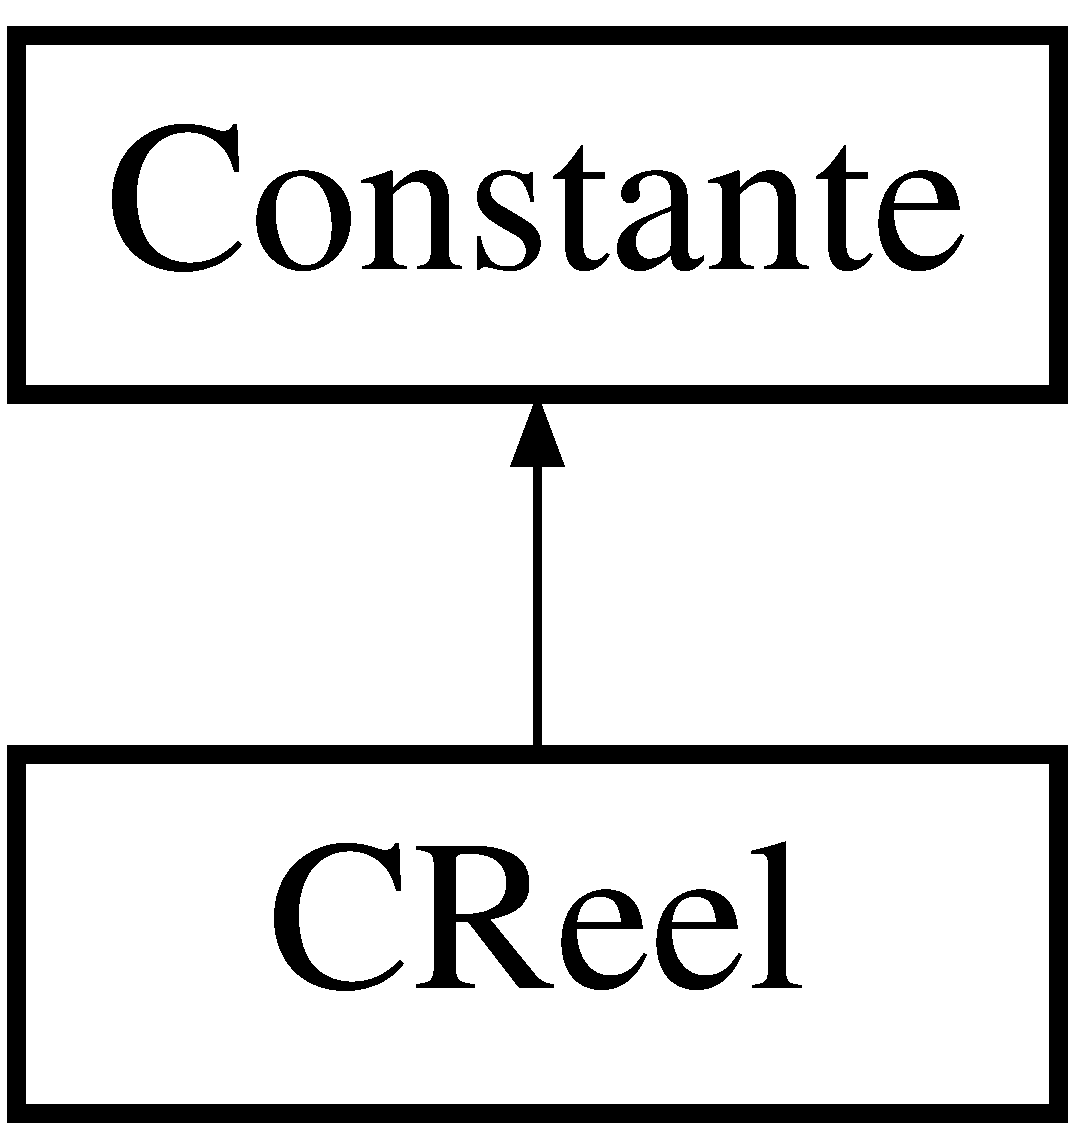
\includegraphics[height=2.000000cm]{class_c_reel}
\end{center}
\end{figure}
\subsection*{Public Member Functions}
\begin{DoxyCompactItemize}
\item 
\hyperlink{class_c_reel_a48315083e4113820ea0c0b52b428b4cb}{C\-Reel} (float v)
\begin{DoxyCompactList}\small\item\em constructeur. \end{DoxyCompactList}\item 
\hyperlink{class_c_reel_a40477248c55c086f5f5b19bfdf4b953c}{C\-Reel} (const \hyperlink{class_c_reel}{C\-Reel} \&c)
\begin{DoxyCompactList}\small\item\em constructeur par copie. \end{DoxyCompactList}\item 
\hyperlink{class_constante}{Constante} $\ast$ \hyperlink{class_c_reel_a7971d82193e3305f266f69547cad8bb7}{get\-Copy} ()
\begin{DoxyCompactList}\small\item\em retourne une copie de la constante \end{DoxyCompactList}\item 
float \hyperlink{class_c_reel_add5e970521e6e7dd6f3374af69826062}{get\-Value} () const 
\begin{DoxyCompactList}\small\item\em retourne la valeur de la constante \end{DoxyCompactList}\item 
void \hyperlink{class_c_reel_ace93771b191f173c66a35ed8ca9f8f61}{set\-Value} (float e)
\begin{DoxyCompactList}\small\item\em affecter une valeur a la constante \end{DoxyCompactList}\item 
Q\-String \hyperlink{class_c_reel_a4f8123c4f5659383d05ead9d02b221ec}{get\-Valueto\-String} () const 
\begin{DoxyCompactList}\small\item\em retourne le contenu de la constante sous forme de texte \end{DoxyCompactList}\item 
\hyperlink{class_constante}{Constante} $\ast$ \hyperlink{class_c_reel_a61a8eb92280d208f9fffa699f9be989f}{operator+} (\hyperlink{class_constante}{Constante} \&c1)
\begin{DoxyCompactList}\small\item\em retourne le resultat de l'operation + entre deux constantes \end{DoxyCompactList}\item 
\hyperlink{class_constante}{Constante} $\ast$ \hyperlink{class_c_reel_abb39aa0b30a2673bdc34b808da836006}{operator-\/} (\hyperlink{class_constante}{Constante} \&c1)
\begin{DoxyCompactList}\small\item\em retourne le resultat de l'operation -\/ entre deux constantes \end{DoxyCompactList}\item 
\hyperlink{class_constante}{Constante} $\ast$ \hyperlink{class_c_reel_ac0730d78556c60bf9824fff423554033}{operator$\ast$} (\hyperlink{class_constante}{Constante} \&c1)
\begin{DoxyCompactList}\small\item\em retourne le resultat de l'operation $\ast$ entre deux constantes \end{DoxyCompactList}\item 
\hyperlink{class_constante}{Constante} $\ast$ \hyperlink{class_c_reel_a12bf069085a82f9d6b99482f538258f9}{operator/} (\hyperlink{class_constante}{Constante} \&c1)
\begin{DoxyCompactList}\small\item\em retourne le resultat de l'operation / entre deux constantes \end{DoxyCompactList}\item 
\hypertarget{class_c_reel_a47f3787b86e124ecf1eb443678afacec}{\hyperlink{class_c_reel_a47f3787b86e124ecf1eb443678afacec}{$\sim$\-C\-Reel} ()}\label{class_c_reel_a47f3787b86e124ecf1eb443678afacec}

\begin{DoxyCompactList}\small\item\em destructeur. \end{DoxyCompactList}\end{DoxyCompactItemize}


\subsection{Detailed Description}
\hyperlink{class_c_reel}{C\-Reel} class. 

classe des types reels 

\subsection{Constructor \& Destructor Documentation}
\hypertarget{class_c_reel_a48315083e4113820ea0c0b52b428b4cb}{\index{C\-Reel@{C\-Reel}!C\-Reel@{C\-Reel}}
\index{C\-Reel@{C\-Reel}!CReel@{C\-Reel}}
\subsubsection[{C\-Reel}]{\setlength{\rightskip}{0pt plus 5cm}C\-Reel\-::\-C\-Reel (
\begin{DoxyParamCaption}
\item[{float}]{v}
\end{DoxyParamCaption}
)\hspace{0.3cm}{\ttfamily [inline]}}}\label{class_c_reel_a48315083e4113820ea0c0b52b428b4cb}


constructeur. 


\begin{DoxyParams}{Parameters}
{\em v} & valeur de la constante \\
\hline
\end{DoxyParams}
\hypertarget{class_c_reel_a40477248c55c086f5f5b19bfdf4b953c}{\index{C\-Reel@{C\-Reel}!C\-Reel@{C\-Reel}}
\index{C\-Reel@{C\-Reel}!CReel@{C\-Reel}}
\subsubsection[{C\-Reel}]{\setlength{\rightskip}{0pt plus 5cm}C\-Reel\-::\-C\-Reel (
\begin{DoxyParamCaption}
\item[{const {\bf C\-Reel} \&}]{c}
\end{DoxyParamCaption}
)\hspace{0.3cm}{\ttfamily [inline]}}}\label{class_c_reel_a40477248c55c086f5f5b19bfdf4b953c}


constructeur par copie. 


\begin{DoxyParams}{Parameters}
{\em c} & reference vers le \hyperlink{class_c_reel}{C\-Reel} a copier \\
\hline
\end{DoxyParams}


\subsection{Member Function Documentation}
\hypertarget{class_c_reel_a7971d82193e3305f266f69547cad8bb7}{\index{C\-Reel@{C\-Reel}!get\-Copy@{get\-Copy}}
\index{get\-Copy@{get\-Copy}!CReel@{C\-Reel}}
\subsubsection[{get\-Copy}]{\setlength{\rightskip}{0pt plus 5cm}{\bf Constante}$\ast$ C\-Reel\-::get\-Copy (
\begin{DoxyParamCaption}
{}
\end{DoxyParamCaption}
)\hspace{0.3cm}{\ttfamily [inline]}, {\ttfamily [virtual]}}}\label{class_c_reel_a7971d82193e3305f266f69547cad8bb7}


retourne une copie de la constante 

\begin{DoxyReturn}{Returns}
pointeur vers une copie de la constante 
\end{DoxyReturn}


Implements \hyperlink{class_constante_addd94a5006b4ed68cc0d1d7b5864e10a}{Constante}.

\hypertarget{class_c_reel_add5e970521e6e7dd6f3374af69826062}{\index{C\-Reel@{C\-Reel}!get\-Value@{get\-Value}}
\index{get\-Value@{get\-Value}!CReel@{C\-Reel}}
\subsubsection[{get\-Value}]{\setlength{\rightskip}{0pt plus 5cm}float C\-Reel\-::get\-Value (
\begin{DoxyParamCaption}
{}
\end{DoxyParamCaption}
) const\hspace{0.3cm}{\ttfamily [inline]}}}\label{class_c_reel_add5e970521e6e7dd6f3374af69826062}


retourne la valeur de la constante 

\begin{DoxyReturn}{Returns}
valeur float 
\end{DoxyReturn}
\hypertarget{class_c_reel_a4f8123c4f5659383d05ead9d02b221ec}{\index{C\-Reel@{C\-Reel}!get\-Valueto\-String@{get\-Valueto\-String}}
\index{get\-Valueto\-String@{get\-Valueto\-String}!CReel@{C\-Reel}}
\subsubsection[{get\-Valueto\-String}]{\setlength{\rightskip}{0pt plus 5cm}Q\-String C\-Reel\-::get\-Valueto\-String (
\begin{DoxyParamCaption}
{}
\end{DoxyParamCaption}
) const\hspace{0.3cm}{\ttfamily [inline]}, {\ttfamily [virtual]}}}\label{class_c_reel_a4f8123c4f5659383d05ead9d02b221ec}


retourne le contenu de la constante sous forme de texte 

\begin{DoxyReturn}{Returns}
Q\-String valeur formatee de la constante 
\end{DoxyReturn}


Implements \hyperlink{class_constante_a93d89080856c972bdebc3619fc957f52}{Constante}.

\hypertarget{class_c_reel_ac0730d78556c60bf9824fff423554033}{\index{C\-Reel@{C\-Reel}!operator$\ast$@{operator$\ast$}}
\index{operator$\ast$@{operator$\ast$}!CReel@{C\-Reel}}
\subsubsection[{operator$\ast$}]{\setlength{\rightskip}{0pt plus 5cm}{\bf Constante} $\ast$ C\-Reel\-::operator$\ast$ (
\begin{DoxyParamCaption}
\item[{{\bf Constante} \&}]{c1}
\end{DoxyParamCaption}
)\hspace{0.3cm}{\ttfamily [virtual]}}}\label{class_c_reel_ac0730d78556c60bf9824fff423554033}


retourne le resultat de l'operation $\ast$ entre deux constantes 


\begin{DoxyParams}{Parameters}
{\em c1} & reference vers le deuxieme operande de type \hyperlink{class_constante}{Constante} \\
\hline
\end{DoxyParams}
\begin{DoxyReturn}{Returns}
un pointeur \hyperlink{class_constante}{Constante} sur le resultat 
\end{DoxyReturn}


Implements \hyperlink{class_constante_ae7c4cf6a493277ec98ae346e13bbf82a}{Constante}.

\hypertarget{class_c_reel_a61a8eb92280d208f9fffa699f9be989f}{\index{C\-Reel@{C\-Reel}!operator+@{operator+}}
\index{operator+@{operator+}!CReel@{C\-Reel}}
\subsubsection[{operator+}]{\setlength{\rightskip}{0pt plus 5cm}{\bf Constante} $\ast$ C\-Reel\-::operator+ (
\begin{DoxyParamCaption}
\item[{{\bf Constante} \&}]{c1}
\end{DoxyParamCaption}
)\hspace{0.3cm}{\ttfamily [virtual]}}}\label{class_c_reel_a61a8eb92280d208f9fffa699f9be989f}


retourne le resultat de l'operation + entre deux constantes 


\begin{DoxyParams}{Parameters}
{\em c1} & reference vers le deuxieme operande de type \hyperlink{class_constante}{Constante} \\
\hline
\end{DoxyParams}
\begin{DoxyReturn}{Returns}
un pointeur \hyperlink{class_constante}{Constante} sur le resultat 
\end{DoxyReturn}


Implements \hyperlink{class_constante_ae1c9e9fa9b3272e37bdb292509741831}{Constante}.

\hypertarget{class_c_reel_abb39aa0b30a2673bdc34b808da836006}{\index{C\-Reel@{C\-Reel}!operator-\/@{operator-\/}}
\index{operator-\/@{operator-\/}!CReel@{C\-Reel}}
\subsubsection[{operator-\/}]{\setlength{\rightskip}{0pt plus 5cm}{\bf Constante} $\ast$ C\-Reel\-::operator-\/ (
\begin{DoxyParamCaption}
\item[{{\bf Constante} \&}]{c1}
\end{DoxyParamCaption}
)\hspace{0.3cm}{\ttfamily [virtual]}}}\label{class_c_reel_abb39aa0b30a2673bdc34b808da836006}


retourne le resultat de l'operation -\/ entre deux constantes 


\begin{DoxyParams}{Parameters}
{\em c1} & reference vers le deuxieme operande de type \hyperlink{class_constante}{Constante} \\
\hline
\end{DoxyParams}
\begin{DoxyReturn}{Returns}
un pointeur \hyperlink{class_constante}{Constante} sur le resultat 
\end{DoxyReturn}


Implements \hyperlink{class_constante_a9d0df3d484c2d87556cb4faa73606862}{Constante}.

\hypertarget{class_c_reel_a12bf069085a82f9d6b99482f538258f9}{\index{C\-Reel@{C\-Reel}!operator/@{operator/}}
\index{operator/@{operator/}!CReel@{C\-Reel}}
\subsubsection[{operator/}]{\setlength{\rightskip}{0pt plus 5cm}{\bf Constante} $\ast$ C\-Reel\-::operator/ (
\begin{DoxyParamCaption}
\item[{{\bf Constante} \&}]{c1}
\end{DoxyParamCaption}
)\hspace{0.3cm}{\ttfamily [virtual]}}}\label{class_c_reel_a12bf069085a82f9d6b99482f538258f9}


retourne le resultat de l'operation / entre deux constantes 


\begin{DoxyParams}{Parameters}
{\em c1} & reference vers le deuxieme operande de type \hyperlink{class_constante}{Constante} \\
\hline
\end{DoxyParams}
\begin{DoxyReturn}{Returns}
un pointeur \hyperlink{class_constante}{Constante} sur le resultat 
\end{DoxyReturn}


Implements \hyperlink{class_constante_af83c6680a11bc9ca5db49a32864151dd}{Constante}.

\hypertarget{class_c_reel_ace93771b191f173c66a35ed8ca9f8f61}{\index{C\-Reel@{C\-Reel}!set\-Value@{set\-Value}}
\index{set\-Value@{set\-Value}!CReel@{C\-Reel}}
\subsubsection[{set\-Value}]{\setlength{\rightskip}{0pt plus 5cm}void C\-Reel\-::set\-Value (
\begin{DoxyParamCaption}
\item[{float}]{e}
\end{DoxyParamCaption}
)\hspace{0.3cm}{\ttfamily [inline]}}}\label{class_c_reel_ace93771b191f173c66a35ed8ca9f8f61}


affecter une valeur a la constante 


\begin{DoxyParams}{Parameters}
{\em e} & valeur float \\
\hline
\end{DoxyParams}


The documentation for this class was generated from the following files\-:\begin{DoxyCompactItemize}
\item 
E\-:/\-Dropbox/\-U\-T\-C/\-G\-I02/\-L\-O21/\-Calculatrice/constante.\-h\item 
E\-:/\-Dropbox/\-U\-T\-C/\-G\-I02/\-L\-O21/\-Calculatrice/constante.\-cpp\end{DoxyCompactItemize}

\hypertarget{class_ecriture_dom}{\section{Ecriture\-Dom Class Reference}
\label{class_ecriture_dom}\index{Ecriture\-Dom@{Ecriture\-Dom}}
}


\hyperlink{class_ecriture_dom}{Ecriture\-Dom} class.  




{\ttfamily \#include $<$ecrituredom.\-h$>$}

\subsection*{Public Member Functions}
\begin{DoxyCompactItemize}
\item 
\hypertarget{class_ecriture_dom_a4e355f1e7181196dc8adc4afc7b525ba}{\hyperlink{class_ecriture_dom_a4e355f1e7181196dc8adc4afc7b525ba}{Ecriture\-Dom} ()}\label{class_ecriture_dom_a4e355f1e7181196dc8adc4afc7b525ba}

\begin{DoxyCompactList}\small\item\em constructeur. \end{DoxyCompactList}\item 
\hypertarget{class_ecriture_dom_a3d4724b95f0d5397d73f911274ea058b}{\hyperlink{class_ecriture_dom_a3d4724b95f0d5397d73f911274ea058b}{$\sim$\-Ecriture\-Dom} ()}\label{class_ecriture_dom_a3d4724b95f0d5397d73f911274ea058b}

\begin{DoxyCompactList}\small\item\em destructeur. \end{DoxyCompactList}\item 
void \hyperlink{class_ecriture_dom_a63eab6fcf0c48a97e00bf7aece94c7c5}{ajoutpile} (Q\-Stack$<$ \hyperlink{class_constante}{Constante} $\ast$ $>$ $\ast$onglet)
\begin{DoxyCompactList}\small\item\em ajoute une pile dans le fichier xml \end{DoxyCompactList}\item 
void \hyperlink{class_ecriture_dom_ac2db3d9c329eab6fbd7afa7f629b6caf}{ajoutpara} (Q\-String type)
\begin{DoxyCompactList}\small\item\em enregistre un parametre de la calculatrice \end{DoxyCompactList}\end{DoxyCompactItemize}


\subsection{Detailed Description}
\hyperlink{class_ecriture_dom}{Ecriture\-Dom} class. 

classe d'ecriture dans un fichier xml de l'etat de la calculette 

\subsection{Member Function Documentation}
\hypertarget{class_ecriture_dom_ac2db3d9c329eab6fbd7afa7f629b6caf}{\index{Ecriture\-Dom@{Ecriture\-Dom}!ajoutpara@{ajoutpara}}
\index{ajoutpara@{ajoutpara}!EcritureDom@{Ecriture\-Dom}}
\subsubsection[{ajoutpara}]{\setlength{\rightskip}{0pt plus 5cm}void Ecriture\-Dom\-::ajoutpara (
\begin{DoxyParamCaption}
\item[{Q\-String}]{type}
\end{DoxyParamCaption}
)}}\label{class_ecriture_dom_ac2db3d9c329eab6fbd7afa7f629b6caf}


enregistre un parametre de la calculatrice 


\begin{DoxyParams}{Parameters}
{\em type} & valeur a ajouter \\
\hline
\end{DoxyParams}
\hypertarget{class_ecriture_dom_a63eab6fcf0c48a97e00bf7aece94c7c5}{\index{Ecriture\-Dom@{Ecriture\-Dom}!ajoutpile@{ajoutpile}}
\index{ajoutpile@{ajoutpile}!EcritureDom@{Ecriture\-Dom}}
\subsubsection[{ajoutpile}]{\setlength{\rightskip}{0pt plus 5cm}void Ecriture\-Dom\-::ajoutpile (
\begin{DoxyParamCaption}
\item[{Q\-Stack$<$ {\bf Constante} $\ast$ $>$ $\ast$}]{onglet}
\end{DoxyParamCaption}
)}}\label{class_ecriture_dom_a63eab6fcf0c48a97e00bf7aece94c7c5}


ajoute une pile dans le fichier xml 


\begin{DoxyParams}{Parameters}
{\em onglet} & pointeur vers la pile a ajouter \\
\hline
\end{DoxyParams}


The documentation for this class was generated from the following files\-:\begin{DoxyCompactItemize}
\item 
E\-:/\-Dropbox/\-U\-T\-C/\-G\-I02/\-L\-O21/\-Calculatrice/ecrituredom.\-h\item 
E\-:/\-Dropbox/\-U\-T\-C/\-G\-I02/\-L\-O21/\-Calculatrice/ecrituredom.\-cpp\end{DoxyCompactItemize}

\hypertarget{class_pile}{\section{Pile Class Reference}
\label{class_pile}\index{Pile@{Pile}}
}


\hyperlink{class_pile}{Pile} class.  




{\ttfamily \#include $<$pile.\-h$>$}

\subsection*{Public Member Functions}
\begin{DoxyCompactItemize}
\item 
\hyperlink{class_pile_a0866305f3090d5c21168c2f3758e7f3c}{Pile} (Q\-Label $\ast$aff, Q\-Radio\-Button $\ast$\-\_\-bt\-Entier, Q\-Radio\-Button $\ast$\-\_\-bt\-Rationnel, Q\-Radio\-Button $\ast$\-\_\-bt\-Degre, Q\-Check\-Box $\ast$\-\_\-bt\-Complexe, int max)
\begin{DoxyCompactList}\small\item\em constructeur. \end{DoxyCompactList}\item 
\hyperlink{class_pile_ab2d1398d675586ff34994e2b109df152}{$\sim$\-Pile} ()
\begin{DoxyCompactList}\small\item\em destructeur. \end{DoxyCompactList}\item 
void \hyperlink{class_pile_a98f3ede0ac9e571149357e2658b2f054}{clone} (\hyperlink{class_pile}{Pile} \&p) const 
\begin{DoxyCompactList}\small\item\em clone la pile dans p. \end{DoxyCompactList}\item 
void \hyperlink{class_pile_a0e6c368c10d31660652f39336c77852c}{set\-Execution\-Commande} (int i)
\begin{DoxyCompactList}\small\item\em affect l'etat d execution des commandes. \end{DoxyCompactList}\item 
void \hyperlink{class_pile_a16b10153da0c61ca74a44426d23f9891}{cast} (\hyperlink{class_constante}{Constante} $\ast$\&cst)
\begin{DoxyCompactList}\small\item\em cast la constante passe en argument en fonction des types actifs \end{DoxyCompactList}\item 
void \hyperlink{class_pile_a67ce82a40340646f59e646199771114d}{afficher} (int taille\-Max)
\begin{DoxyCompactList}\small\item\em affiche les taille\-Max premiers elements de la pile \end{DoxyCompactList}\item 
\hypertarget{class_pile_af8efea7a91f6403eab295577004ae620}{void \hyperlink{class_pile_af8efea7a91f6403eab295577004ae620}{annuler} ()}\label{class_pile_af8efea7a91f6403eab295577004ae620}

\begin{DoxyCompactList}\small\item\em annule la derniere commande \end{DoxyCompactList}\item 
\hypertarget{class_pile_a36b0ff28bf644cebe2d336ebbb0a07ac}{void \hyperlink{class_pile_a36b0ff28bf644cebe2d336ebbb0a07ac}{retablir} ()}\label{class_pile_a36b0ff28bf644cebe2d336ebbb0a07ac}

\begin{DoxyCompactList}\small\item\em retabli la derniere commande \end{DoxyCompactList}\item 
void \hyperlink{class_pile_a03ccb5ba35c7d4264612b8ec922985a8}{save\-Commande} (\hyperlink{class_commande}{Commande} $\ast$c)
\begin{DoxyCompactList}\small\item\em enregistre une commande \end{DoxyCompactList}\item 
\hypertarget{class_pile_a2c9967dc8f5dcb4372475dee52ed64c6}{void \hyperlink{class_pile_a2c9967dc8f5dcb4372475dee52ed64c6}{swap} ()}\label{class_pile_a2c9967dc8f5dcb4372475dee52ed64c6}

\begin{DoxyCompactList}\small\item\em effectue operation swap sur la pile \end{DoxyCompactList}\item 
\hypertarget{class_pile_a955a5f169fe3e25690e08ac1b32c0228}{void \hyperlink{class_pile_a955a5f169fe3e25690e08ac1b32c0228}{sum} ()}\label{class_pile_a955a5f169fe3e25690e08ac1b32c0228}

\begin{DoxyCompactList}\small\item\em effectue operation sum sur la pile \end{DoxyCompactList}\item 
\hypertarget{class_pile_a3539e61bf44a2aa5929c771ef0e45d4b}{void \hyperlink{class_pile_a3539e61bf44a2aa5929c771ef0e45d4b}{mean} ()}\label{class_pile_a3539e61bf44a2aa5929c771ef0e45d4b}

\begin{DoxyCompactList}\small\item\em effectue operation mean sur la pile \end{DoxyCompactList}\item 
\hypertarget{class_pile_aa3991438f190580607d7bbbd50ecc0c3}{void \hyperlink{class_pile_aa3991438f190580607d7bbbd50ecc0c3}{clear} ()}\label{class_pile_aa3991438f190580607d7bbbd50ecc0c3}

\begin{DoxyCompactList}\small\item\em effectue operation clear sur la pile \end{DoxyCompactList}\item 
\hypertarget{class_pile_a081f7843d01cae1f0f7be7d92e46d5d2}{void \hyperlink{class_pile_a081f7843d01cae1f0f7be7d92e46d5d2}{dup} ()}\label{class_pile_a081f7843d01cae1f0f7be7d92e46d5d2}

\begin{DoxyCompactList}\small\item\em effectue operation dup sur la pile \end{DoxyCompactList}\item 
\hypertarget{class_pile_a7488ed257c6ceb16ed57a9fffb0726d5}{void \hyperlink{class_pile_a7488ed257c6ceb16ed57a9fffb0726d5}{drop} ()}\label{class_pile_a7488ed257c6ceb16ed57a9fffb0726d5}

\begin{DoxyCompactList}\small\item\em effectue operation drop sur la pile \end{DoxyCompactList}\item 
\hypertarget{class_pile_a94a0b5e00d490a838cdbd4b2cd141e76}{void \hyperlink{class_pile_a94a0b5e00d490a838cdbd4b2cd141e76}{f\-Addition} ()}\label{class_pile_a94a0b5e00d490a838cdbd4b2cd141e76}

\begin{DoxyCompactList}\small\item\em effectue operation Addition sur la pile \end{DoxyCompactList}\item 
\hypertarget{class_pile_ad296bc1695546ffa4a412143c16c9b28}{void \hyperlink{class_pile_ad296bc1695546ffa4a412143c16c9b28}{f\-Soustraction} ()}\label{class_pile_ad296bc1695546ffa4a412143c16c9b28}

\begin{DoxyCompactList}\small\item\em effectue operation Soustraction sur la pile \end{DoxyCompactList}\item 
\hypertarget{class_pile_ab3c86545524e1d4f1967bee9f98f7073}{void \hyperlink{class_pile_ab3c86545524e1d4f1967bee9f98f7073}{f\-Multiplication} ()}\label{class_pile_ab3c86545524e1d4f1967bee9f98f7073}

\begin{DoxyCompactList}\small\item\em effectue operation Multiplication sur la pile \end{DoxyCompactList}\item 
\hypertarget{class_pile_ac07c42f15aff4fd36d939478f4a8ba74}{void \hyperlink{class_pile_ac07c42f15aff4fd36d939478f4a8ba74}{f\-Division} ()}\label{class_pile_ac07c42f15aff4fd36d939478f4a8ba74}

\begin{DoxyCompactList}\small\item\em effectue operation Division sur la pile \end{DoxyCompactList}\item 
\hypertarget{class_pile_a1ea4c2ae05a4fc10dea3741e5ad98eca}{void \hyperlink{class_pile_a1ea4c2ae05a4fc10dea3741e5ad98eca}{f\-P\-O\-W} ()}\label{class_pile_a1ea4c2ae05a4fc10dea3741e5ad98eca}

\begin{DoxyCompactList}\small\item\em effectue fonction puissance (entier, rationnel, reel) \end{DoxyCompactList}\item 
\hypertarget{class_pile_a2730fae99b4c5179b79cd9f124429ad9}{void \hyperlink{class_pile_a2730fae99b4c5179b79cd9f124429ad9}{f\-M\-O\-D} ()}\label{class_pile_a2730fae99b4c5179b79cd9f124429ad9}

\begin{DoxyCompactList}\small\item\em effectue fonction modulo (entier) \end{DoxyCompactList}\item 
\hypertarget{class_pile_a2c8f3f9e11497dad8fdd1d426abe2bb8}{void \hyperlink{class_pile_a2c8f3f9e11497dad8fdd1d426abe2bb8}{f\-S\-I\-G\-N} ()}\label{class_pile_a2c8f3f9e11497dad8fdd1d426abe2bb8}

\begin{DoxyCompactList}\small\item\em effectue fonction inversion du signe (entier, rationnel, reel, complexe) \end{DoxyCompactList}\item 
\hypertarget{class_pile_a7c57a5b96416585b364551183fac9d5b}{void \hyperlink{class_pile_a7c57a5b96416585b364551183fac9d5b}{f\-S\-I\-N} ()}\label{class_pile_a7c57a5b96416585b364551183fac9d5b}

\begin{DoxyCompactList}\small\item\em effectue fonction sinus (entier, rationnel, reel) \end{DoxyCompactList}\item 
\hypertarget{class_pile_aabc4b3288a748cc5fc20e3eafe03e418}{void \hyperlink{class_pile_aabc4b3288a748cc5fc20e3eafe03e418}{f\-C\-O\-S} ()}\label{class_pile_aabc4b3288a748cc5fc20e3eafe03e418}

\begin{DoxyCompactList}\small\item\em effectue fonction cosinus (entier, rationnel, reel) \end{DoxyCompactList}\item 
\hypertarget{class_pile_a8a3fadda0bf8ca55861fc17d15573b18}{void \hyperlink{class_pile_a8a3fadda0bf8ca55861fc17d15573b18}{f\-T\-A\-N} ()}\label{class_pile_a8a3fadda0bf8ca55861fc17d15573b18}

\begin{DoxyCompactList}\small\item\em effectue fonction tangente (entier, rationnel, reel) \end{DoxyCompactList}\item 
\hypertarget{class_pile_aef8fca3177bec1021a5f85de9df3cfa2}{void \hyperlink{class_pile_aef8fca3177bec1021a5f85de9df3cfa2}{f\-S\-I\-N\-H} ()}\label{class_pile_aef8fca3177bec1021a5f85de9df3cfa2}

\begin{DoxyCompactList}\small\item\em effectue fonction sinus hyperbolique (entier, rationnel, reel) \end{DoxyCompactList}\item 
\hypertarget{class_pile_a41920a6c8810da368b65d74ccab119bc}{void \hyperlink{class_pile_a41920a6c8810da368b65d74ccab119bc}{f\-C\-O\-S\-H} ()}\label{class_pile_a41920a6c8810da368b65d74ccab119bc}

\begin{DoxyCompactList}\small\item\em effectue fonction cosinus hyperbolique (entier, rationnel, reel) \end{DoxyCompactList}\item 
\hypertarget{class_pile_a3502ad2b3d47c01fed500f45a63d73aa}{void \hyperlink{class_pile_a3502ad2b3d47c01fed500f45a63d73aa}{f\-T\-A\-N\-H} ()}\label{class_pile_a3502ad2b3d47c01fed500f45a63d73aa}

\begin{DoxyCompactList}\small\item\em effectue fonction tangente hyperbolique (entier, rationnel, reel) \end{DoxyCompactList}\item 
\hypertarget{class_pile_ac2dbfceac12846d16ab86225e5f95e19}{void \hyperlink{class_pile_ac2dbfceac12846d16ab86225e5f95e19}{f\-L\-N} ()}\label{class_pile_ac2dbfceac12846d16ab86225e5f95e19}

\begin{DoxyCompactList}\small\item\em effectue fonction logarithme neperien (entier, rationnel, reel) \end{DoxyCompactList}\item 
\hypertarget{class_pile_afb45811f5a215c144bff16598c5e8054}{void \hyperlink{class_pile_afb45811f5a215c144bff16598c5e8054}{f\-L\-O\-G} ()}\label{class_pile_afb45811f5a215c144bff16598c5e8054}

\begin{DoxyCompactList}\small\item\em effectue fonction logarithme decimal (entier, rationnel, reel) \end{DoxyCompactList}\item 
\hypertarget{class_pile_ab832ceba68c7a40cc5bd40045dca3dce}{void \hyperlink{class_pile_ab832ceba68c7a40cc5bd40045dca3dce}{f\-I\-N\-V} ()}\label{class_pile_ab832ceba68c7a40cc5bd40045dca3dce}

\begin{DoxyCompactList}\small\item\em effectue fonction inverse (entier, rationnel, reel) \end{DoxyCompactList}\item 
\hypertarget{class_pile_af1480988b888425a246a1f5368824659}{void \hyperlink{class_pile_af1480988b888425a246a1f5368824659}{f\-S\-Q\-R\-T} ()}\label{class_pile_af1480988b888425a246a1f5368824659}

\begin{DoxyCompactList}\small\item\em effectue fonction racine carre (entier, rationnel, reel) \end{DoxyCompactList}\item 
\hypertarget{class_pile_af39fcfe00509c9d155e8851d7b7fd2f7}{void \hyperlink{class_pile_af39fcfe00509c9d155e8851d7b7fd2f7}{f\-S\-Q\-R} ()}\label{class_pile_af39fcfe00509c9d155e8851d7b7fd2f7}

\begin{DoxyCompactList}\small\item\em effectue fonction carre (entier, rationnel, reel, complexe) \end{DoxyCompactList}\item 
\hypertarget{class_pile_adc93d5906457e6d9337e0e763c39f70b}{void \hyperlink{class_pile_adc93d5906457e6d9337e0e763c39f70b}{f\-C\-U\-B\-E} ()}\label{class_pile_adc93d5906457e6d9337e0e763c39f70b}

\begin{DoxyCompactList}\small\item\em effectue fonction cube (entier, rationnel, reel, complexe) \end{DoxyCompactList}\item 
\hypertarget{class_pile_a582a24a17a82fc63985900765b0499b4}{void \hyperlink{class_pile_a582a24a17a82fc63985900765b0499b4}{fact} ()}\label{class_pile_a582a24a17a82fc63985900765b0499b4}

\begin{DoxyCompactList}\small\item\em effectue factorielle (entier) \end{DoxyCompactList}\item 
\hypertarget{class_pile_a7e676351f3811c37c4866071162050de}{void \hyperlink{class_pile_a7e676351f3811c37c4866071162050de}{f\-E\-V\-A\-L} ()}\label{class_pile_a7e676351f3811c37c4866071162050de}

\begin{DoxyCompactList}\small\item\em evaluation d'une expression (Expression) \end{DoxyCompactList}\end{DoxyCompactItemize}
\subsection*{Public Attributes}
\begin{DoxyCompactItemize}
\item 
\hypertarget{class_pile_aa7b32a34ea2b81420d851dfd344d6580}{Q\-Label $\ast$ \hyperlink{class_pile_aa7b32a34ea2b81420d851dfd344d6580}{affichage}}\label{class_pile_aa7b32a34ea2b81420d851dfd344d6580}

\begin{DoxyCompactList}\small\item\em Pointeur vers l'affichage du texte. \end{DoxyCompactList}\end{DoxyCompactItemize}


\subsection{Detailed Description}
\hyperlink{class_pile}{Pile} class. 

pile contenant les Constantes 

\subsection{Constructor \& Destructor Documentation}
\hypertarget{class_pile_a0866305f3090d5c21168c2f3758e7f3c}{\index{Pile@{Pile}!Pile@{Pile}}
\index{Pile@{Pile}!Pile@{Pile}}
\subsubsection[{Pile}]{\setlength{\rightskip}{0pt plus 5cm}Pile\-::\-Pile (
\begin{DoxyParamCaption}
\item[{Q\-Label $\ast$}]{aff, }
\item[{Q\-Radio\-Button $\ast$}]{\-\_\-bt\-Entier, }
\item[{Q\-Radio\-Button $\ast$}]{\-\_\-bt\-Rationnel, }
\item[{Q\-Radio\-Button $\ast$}]{\-\_\-bt\-Degre, }
\item[{Q\-Check\-Box $\ast$}]{\-\_\-bt\-Complexe, }
\item[{int}]{max}
\end{DoxyParamCaption}
)}}\label{class_pile_a0866305f3090d5c21168c2f3758e7f3c}


constructeur. 


\begin{DoxyParams}{Parameters}
{\em aff} & pointeur sur l'afficheur de la pile \\
\hline
{\em \-\_\-bt\-Entier} & pointeur vers radio\-Button Entier \\
\hline
{\em \-\_\-bt\-Rationnel} & pointeur vers radio\-Button Rationnel \\
\hline
{\em \-\_\-bt\-Degre} & pointeur vers radio\-Button Degre \\
\hline
{\em \-\_\-bt\-Complexe} & pointeur vers radio\-Button Complexe \\
\hline
{\em max} & nombre d'elements a afficher \\
\hline
\end{DoxyParams}
\hypertarget{class_pile_ab2d1398d675586ff34994e2b109df152}{\index{Pile@{Pile}!$\sim$\-Pile@{$\sim$\-Pile}}
\index{$\sim$\-Pile@{$\sim$\-Pile}!Pile@{Pile}}
\subsubsection[{$\sim$\-Pile}]{\setlength{\rightskip}{0pt plus 5cm}Pile\-::$\sim$\-Pile (
\begin{DoxyParamCaption}
{}
\end{DoxyParamCaption}
)}}\label{class_pile_ab2d1398d675586ff34994e2b109df152}


destructeur. 

destruction de l'ensemble des commandes et des constantes 

\subsection{Member Function Documentation}
\hypertarget{class_pile_a67ce82a40340646f59e646199771114d}{\index{Pile@{Pile}!afficher@{afficher}}
\index{afficher@{afficher}!Pile@{Pile}}
\subsubsection[{afficher}]{\setlength{\rightskip}{0pt plus 5cm}void Pile\-::afficher (
\begin{DoxyParamCaption}
\item[{int}]{taille\-Max}
\end{DoxyParamCaption}
)}}\label{class_pile_a67ce82a40340646f59e646199771114d}


affiche les taille\-Max premiers elements de la pile 


\begin{DoxyParams}{Parameters}
{\em taille\-Max} & integer nombre d element a afficher \\
\hline
\end{DoxyParams}
\hypertarget{class_pile_a16b10153da0c61ca74a44426d23f9891}{\index{Pile@{Pile}!cast@{cast}}
\index{cast@{cast}!Pile@{Pile}}
\subsubsection[{cast}]{\setlength{\rightskip}{0pt plus 5cm}void Pile\-::cast (
\begin{DoxyParamCaption}
\item[{{\bf Constante} $\ast$\&}]{cst}
\end{DoxyParamCaption}
)}}\label{class_pile_a16b10153da0c61ca74a44426d23f9891}


cast la constante passe en argument en fonction des types actifs 


\begin{DoxyParams}{Parameters}
{\em cst} & constante a caster \\
\hline
\end{DoxyParams}
\hypertarget{class_pile_a98f3ede0ac9e571149357e2658b2f054}{\index{Pile@{Pile}!clone@{clone}}
\index{clone@{clone}!Pile@{Pile}}
\subsubsection[{clone}]{\setlength{\rightskip}{0pt plus 5cm}void Pile\-::clone (
\begin{DoxyParamCaption}
\item[{{\bf Pile} \&}]{p}
\end{DoxyParamCaption}
) const}}\label{class_pile_a98f3ede0ac9e571149357e2658b2f054}


clone la pile dans p. 


\begin{DoxyParams}{Parameters}
{\em p} & pile copie \\
\hline
\end{DoxyParams}
\hypertarget{class_pile_a03ccb5ba35c7d4264612b8ec922985a8}{\index{Pile@{Pile}!save\-Commande@{save\-Commande}}
\index{save\-Commande@{save\-Commande}!Pile@{Pile}}
\subsubsection[{save\-Commande}]{\setlength{\rightskip}{0pt plus 5cm}void Pile\-::save\-Commande (
\begin{DoxyParamCaption}
\item[{{\bf Commande} $\ast$}]{c}
\end{DoxyParamCaption}
)}}\label{class_pile_a03ccb5ba35c7d4264612b8ec922985a8}


enregistre une commande 


\begin{DoxyParams}{Parameters}
{\em c} & Pointeur de commande a enregistrer \\
\hline
\end{DoxyParams}
\hypertarget{class_pile_a0e6c368c10d31660652f39336c77852c}{\index{Pile@{Pile}!set\-Execution\-Commande@{set\-Execution\-Commande}}
\index{set\-Execution\-Commande@{set\-Execution\-Commande}!Pile@{Pile}}
\subsubsection[{set\-Execution\-Commande}]{\setlength{\rightskip}{0pt plus 5cm}void Pile\-::set\-Execution\-Commande (
\begin{DoxyParamCaption}
\item[{int}]{i}
\end{DoxyParamCaption}
)\hspace{0.3cm}{\ttfamily [inline]}}}\label{class_pile_a0e6c368c10d31660652f39336c77852c}


affect l'etat d execution des commandes. 


\begin{DoxyParams}{Parameters}
{\em i} & integer etat \\
\hline
\end{DoxyParams}
\begin{DoxySeeAlso}{See also}
execution\-Commande 
\end{DoxySeeAlso}


The documentation for this class was generated from the following files\-:\begin{DoxyCompactItemize}
\item 
E\-:/\-Dropbox/\-U\-T\-C/\-G\-I02/\-L\-O21/\-Calculatrice/pile.\-h\item 
E\-:/\-Dropbox/\-U\-T\-C/\-G\-I02/\-L\-O21/\-Calculatrice/pile.\-cpp\end{DoxyCompactItemize}

\hypertarget{class_xml___dom}{\section{Xml\-\_\-\-Dom Class Reference}
\label{class_xml___dom}\index{Xml\-\_\-\-Dom@{Xml\-\_\-\-Dom}}
}


\hyperlink{class_xml___dom}{Xml\-\_\-\-Dom} class.  




{\ttfamily \#include $<$xml\-\_\-dom.\-h$>$}

\subsection*{Public Member Functions}
\begin{DoxyCompactItemize}
\item 
\hyperlink{class_xml___dom_a061368f8b4562aaa21f4a2f59cf1c4e5}{Xml\-\_\-\-Dom} (\hyperlink{class_calculatrice}{Calculatrice} $\ast$c)
\begin{DoxyCompactList}\small\item\em constructeur. \end{DoxyCompactList}\item 
\hypertarget{class_xml___dom_a541d7cc499b7c458c0a86a3766a1f68d}{\hyperlink{class_xml___dom_a541d7cc499b7c458c0a86a3766a1f68d}{$\sim$\-Xml\-\_\-\-Dom} ()}\label{class_xml___dom_a541d7cc499b7c458c0a86a3766a1f68d}

\begin{DoxyCompactList}\small\item\em destructeur. \end{DoxyCompactList}\end{DoxyCompactItemize}


\subsection{Detailed Description}
\hyperlink{class_xml___dom}{Xml\-\_\-\-Dom} class. 

Classe de lecture de fichier X\-M\-L 

\subsection{Constructor \& Destructor Documentation}
\hypertarget{class_xml___dom_a061368f8b4562aaa21f4a2f59cf1c4e5}{\index{Xml\-\_\-\-Dom@{Xml\-\_\-\-Dom}!Xml\-\_\-\-Dom@{Xml\-\_\-\-Dom}}
\index{Xml\-\_\-\-Dom@{Xml\-\_\-\-Dom}!Xml_Dom@{Xml\-\_\-\-Dom}}
\subsubsection[{Xml\-\_\-\-Dom}]{\setlength{\rightskip}{0pt plus 5cm}Xml\-\_\-\-Dom\-::\-Xml\-\_\-\-Dom (
\begin{DoxyParamCaption}
\item[{{\bf Calculatrice} $\ast$}]{c}
\end{DoxyParamCaption}
)}}\label{class_xml___dom_a061368f8b4562aaa21f4a2f59cf1c4e5}


constructeur. 


\begin{DoxyParams}{Parameters}
{\em c} & pointeur sur la fenetre de la calculatrice lit puis construit les piles a l'ouverture de l'application \\
\hline
\end{DoxyParams}


The documentation for this class was generated from the following files\-:\begin{DoxyCompactItemize}
\item 
E\-:/\-Dropbox/\-U\-T\-C/\-G\-I02/\-L\-O21/\-Calculatrice/xml\-\_\-dom.\-h\item 
E\-:/\-Dropbox/\-U\-T\-C/\-G\-I02/\-L\-O21/\-Calculatrice/xml\-\_\-dom.\-cpp\end{DoxyCompactItemize}

\printindex
\end{document}
